\documentclass[12pt]{report}
\usepackage{hyperref}
\usepackage[pdftex]{graphicx}
\usepackage[normalem]{ulem}
\usepackage[utf8]{inputenc}
\usepackage[english,frenchb,francais]{babel}
\usepackage[T1]{fontenc}
\usepackage{hyperref}
\usepackage{geometry}
\usepackage{wrapfig}
\geometry{hmargin=1.5cm,vmargin=1.5cm}

\begin{document}
  \begin{titlepage}
    \centering
        \vfill
        {\rule{\linewidth}{.5pt}
        \huge
            Optimisation par algorithme génétique\\
          \large
            Influence du paramétrage\\
          \rule{\linewidth}{.5pt}
            \vskip2cm
            Swan Launay - Gabriel Vaubaillon\\
        }
        \vfill
        
\includegraphics[height=1.7cm]{logo/polytech.jpg}
        \hfill
        
\includegraphics[height=1.7cm]{logo/usmb.png}
  \end{titlepage}
  \pagenumbering{Roman}
  \chapter{Préambule}
    \section{Remerciements}
      Ce rapport représente l'aboutissement d'un projet de 40 heures qui s'est déroulé entre octobre 2018 et avril 2019. Nous tenons tout d'abord à remercier Gilles Fraisse pour son soutien, sa pédagogie, mais aussi pour le temps qu'il a passé à nous accompagner.

      Nous tenons aussi à remercier l'Université Savoie Mont Blanc (USMB) pour la mise à disposition des documents nécessaires à la réalisation de ce projet par le biais, notamment, de la bibliothèque universitaire.

      Nous remercions enfin Polytech Annecy - Chambéry pour nous avoir permis d'effectuer ce projet sur notre temps de travail universitaire et plus globalement pour nous avoir proposé un travail de ce type.

    \section{Résumé}
      L'optimisation par algorithme génétique permet d'obtenir de bonnes approximations de résolutions pour différents problèmes (avec un ou plusieurs objectifs). De façon générale, les algorithmes génétiques sont construits de telle façon à ce que l'on puisse faire varier certains paramètres. C'est ces mêmes paramètres qui vont déterminer la qualité et la fiabilité du résultat, mais aussi qui vont faire varier de façon plus ou moins significative le temps de résolution. Il s'agit alors de trouver un juste milieu entre le temps résolution et la fiabilité du résultat.

  \chapter{Introduction}
    Selon la \emph{Théorie de l'évolution} \cite{darwin} de Charles Darwin, l'évolution des espèces est issue de mutations aléatoires qui surviennent lors de la conception d'une nouvelle génération d'individus. Si cette mutation permet à l'individu d'être plus adapté à son milieu de vie, alors il aura plus de chances d'atteindre l'âge adulte et d'engendrer une nouvelle génération.
    Les algorithmes génétiques sont une application directe du darwinisme à l'informatique.\\
    De nos jours, ces algorithmes permettent de résoudre des problèmes d'optimisation, c'est-à-dire de maximiser ou de minimiser numériquement une ou plusieurs fonctions.
    La branche des mathématiques qu'est l'optimisation est un élément central dans le monde de l'ingénierie ou on cherche dans de très nombreux cas à minimiser plusieurs problèmes à la fois et à obtenir une solution de qualité dans un laps de temps court.\\
    Ce rapport présente deux types d'algorithme génétique différents, le premier est adapté à une optimisation mono-objectif (un seul problème), alors que l'autre l'est pour des problèmes multiobjectifs. Pour chacun des deux algorithmes nous détaillerons à la fois le principe de résolution, mais aussi l'influence du paramétrage.

  \tableofcontents
  \chapter{Optimisation à objectif unique}
    \pagenumbering{arabic}
    \begin{description}
      \item[Définition :] on dit d'un algorithme qu'il est à objectif unique (mono-objectif) s'il ne cherche à optimiser qu'une seule fonction. Dans le cas d'une optimisation qui comprend plusieurs fonctions on parle alors d'algorithmes multiobjectifs.
    \end{description}
    \section{Algorithme}
      \subsection{Principe}
        \begin{wrapfigure}[22]{r}{6cm}
        \centering
        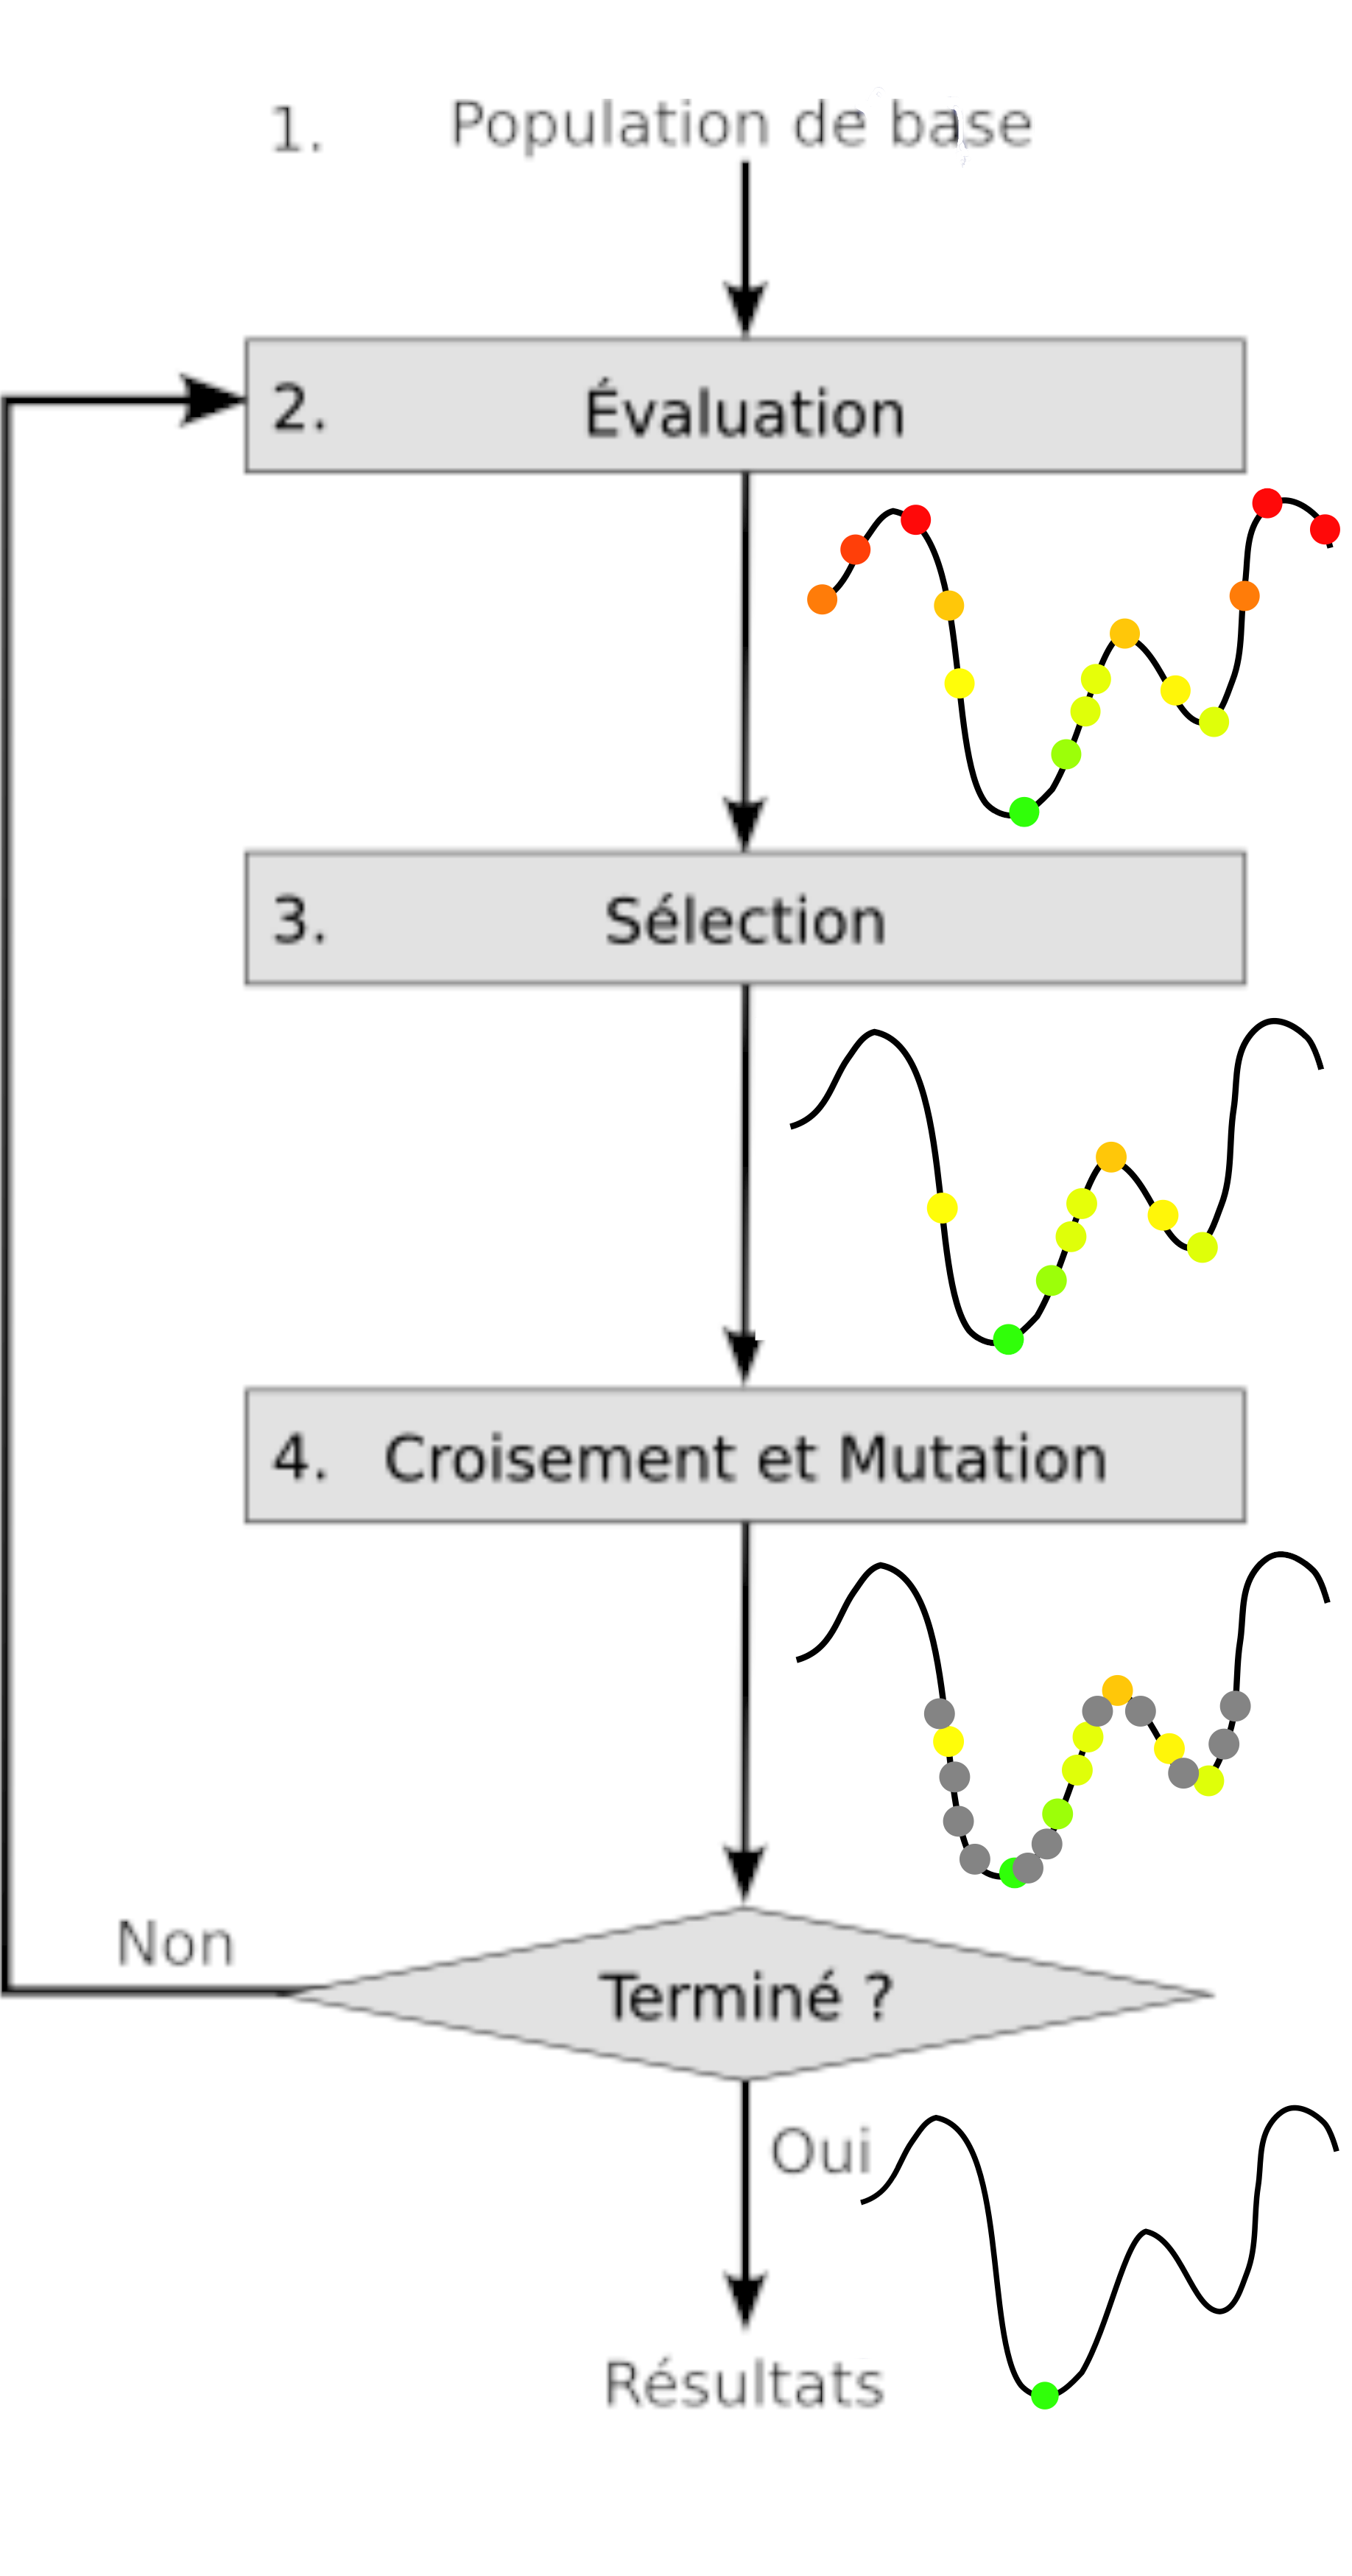
\includegraphics[width=5cm]{img/schema_algo_single.png}
        \caption{Fonctionnement type d'un algorithme génétique}
        \label{logi}
        \end{wrapfigure}
        Hormis quelques variations dans leur conception, les algorithmes génétiques ont pratiquement tous le même principe de fonctionnement.
        Le logigramme ci-joint \ref{logi} illustre le fonctionnement de base d'un algorithme mono-objectif.
        On commence par générer de façon aléatoire une population de base qui servira d'initialisation de notre algorithme.
        Chaque individu de cette population est alors évalué, on lui attribue une valeur qui va déterminer sa position par rapport à la solution optimale recherchée (ici le minimum de la fonction).
        Une sélection est ensuite effectuée en gardant les meilleurs résultats, mais aussi en gardant un certain pourcentage de valeurs considérées comme de moyenne/faible qualité. Cette dernière opération permet entre autres à l'algorithme de ne pas tomber dans un extremum local.
        À partir de cette sélection, l'algorithme va procéder à deux étapes :

        Le croisement (Crossover) :
          il consiste à partager (croiser) les particularités de deux individus parents pour engendrer une nouvelle population d'individus conservant ces mêmes particularités. À noter qu'il existe plusieurs méthodes de croisement (linéaire, à n points, ... etc) qui ont chacune leurs particularités. Dans notre cas c'est le croisement à 3 points de rotation qui est utilisé, son fonctionnement est expliqué par la figure \ref{sch_crossover}.
          \emph{Remarque : On retrouve cette opération en biologie sous le nom de "brassage génétique" qui illustre le principe d'héridité de la théorie de Darwin \cite{darwin}.}
          \begin{figure}[h]
            \centering
            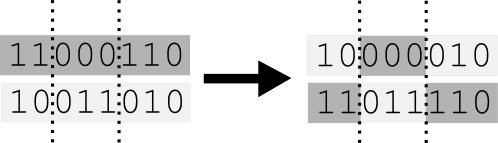
\includegraphics{img/crossover.png}
            \caption{Analogie binaire d'un croisement à 3 points de rotation}
            \label{sch_crossover}
          \end{figure}

        La mutation \cite{wiki6} :
          contrairement au croisement qui conserve les particularités des individus au cours des générations, la mutation altère certains individus de manière aléatoire. Cette opération complète l'opération de sélection précédemment évoquée afin d'éviter de tomber dans un extremum local.
          \emph{Remarque : cette opération illustre le principe de variation de la théorie de Darwin \cite{darwin}.}

    \section{Optimisation unidimensionnelle / multidimensionnelle}
      Bien que l'optimisation mono-objectif signifie l'optimisation d'un seul problème, ce problème peut tout de même comporter plusieurs variables, on parle alors d'optimisation multidimensionnelle $(\mathbb{R}^n \rightarrow \mathbb{R})$. Il est possible de représenter graphiquement de tels problèmes jusqu'à une dimension égale à 2 (Voir figure \ref{ex_r2}).

      \begin{figure}[h]
        \begin{minipage}[c]{.46\linewidth}
            \centering
            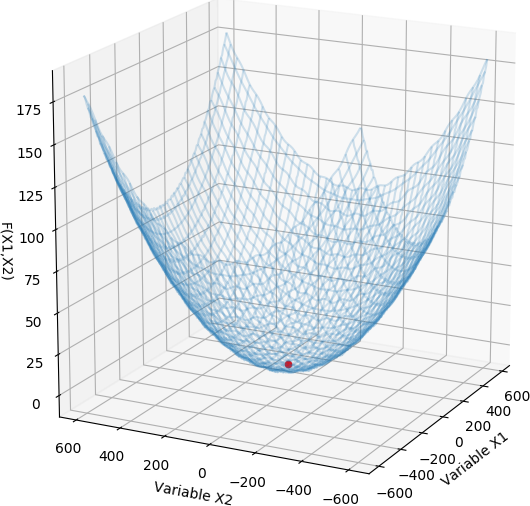
\includegraphics[width=6cm]{img/3,2.png}
            \caption{Fonction Griwank \cite{wiki5} en bleu, solution de l'algorithme en rouge}
            \label{ex_r2}
        \end{minipage}
        \hfill%
        \begin{minipage}[c]{.46\linewidth}
            \centering
            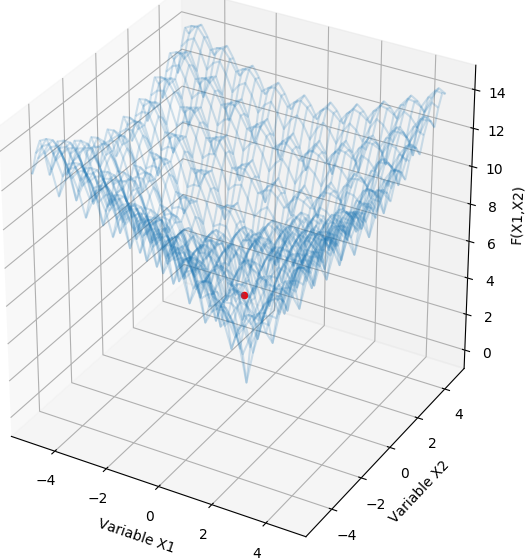
\includegraphics[width=6cm]{img/ackley.png}
            \caption{Fonction Ackley \cite{wiki5}}
            \label{ackley}
        \end{minipage}
      \end{figure}

    \section{Influence du paramétrage }

      Lors de son exécution, un algorithme génétique est soumis à un paramétrage préalablement défini par l'utilisateur. Ce paramétrage va agir sur le comportement et sur la capacité de l'algorithme à trouver des solutions de qualité. Dans le cadre de ce projet, c'est  l'influence de ce paramétrage qui nous intéresse, on cherche donc à faire varier les paramètres pour se rendre compte de l'influence qu'ils ont sur l'algorithme.

      \subsection{Protocole}
        \begin{itemize}
          \item Dans cette partie la fonction dont on cherche le minimum se nomme Ackley et est définie tel que :
          $$
          \left\{
            \begin{array}{ll}
               \forall x,y \in [-5,5], f(x,y) = -20 * e^{-0.2\sqrt{0.5(x^2+y^2)}} $$ \\
               Solution de référence : f(0,0) = 0 $$
            \end{array}
          \right.
          $$
          \item Afin d'étudier l'influence des paramètres sur la résolution du problème nous avons réalisé un programme en python qui nous permet de récupérer l'évolution de la solution en fonction du nombre de générations. On fait ensuite varier soit la taille de la population, soit la probabilité de croisement, soit la probabilité de mutation. Nous obtenons alors un ensemble de courbes où chacune est associée à une valeur du paramètre sélectionné. Nous pouvons ainsi regarder l'évolution des courbes et déterminer l'influence du paramétrage sur la qualité de la solution.

          On définit l'efficacité de la résolution par rapport à la qualité de la solution obtenue et le nombre de générations nécessaires pour obtenir un résultat convenable. Afin d'obtenir ces résultats notre programme est séparé en plusieurs morceaux (Voir figure \ref{logi}).

          \begin{enumerate}
          \item Dans un premier temps il nous faut la résolution du problème en elle-même. Nous faisons cela avec la bibliothèque Python Inspyred \cite{inspyred} qui offre de nombreuses procédures/fonctions destinées à la programmation génétique. Lors d'une résolution du problème nous donnons à l'algorithme plusieurs paramètres : le nombre de générations, la taille de population, la probabilité de croisement et la probabilité de mutation.

          Nous voulons donc tracer des courbes avec différentes valeurs de paramètres pour les comparer, notre programme fait alors varier automatiquement le paramètre choisi et génère la courbe des solutions en fonction du nombre de générations. On stocke ensuite les courbes pour chaque valeur de variation dans un fichier.
          \emph{Remarque : Afin de passer à l'étape suivante cette partie est réalisé plusieurs fois dans les même conditions.}

          \item Dans un second temps, afin d'obtenir des courbes exploitables on réalise la moyenne de tous les fichiers obtenus pour un même problème.

          \item Et enfin, dans un troisième et dernier temps on procède au lissage des courbes moyennes précédemment générées en faisant une seconde moyenne directement sur les valeurs de chaque courbe.
        \end{enumerate}
        \end{itemize}
          \begin{figure}[!]
            \centering
            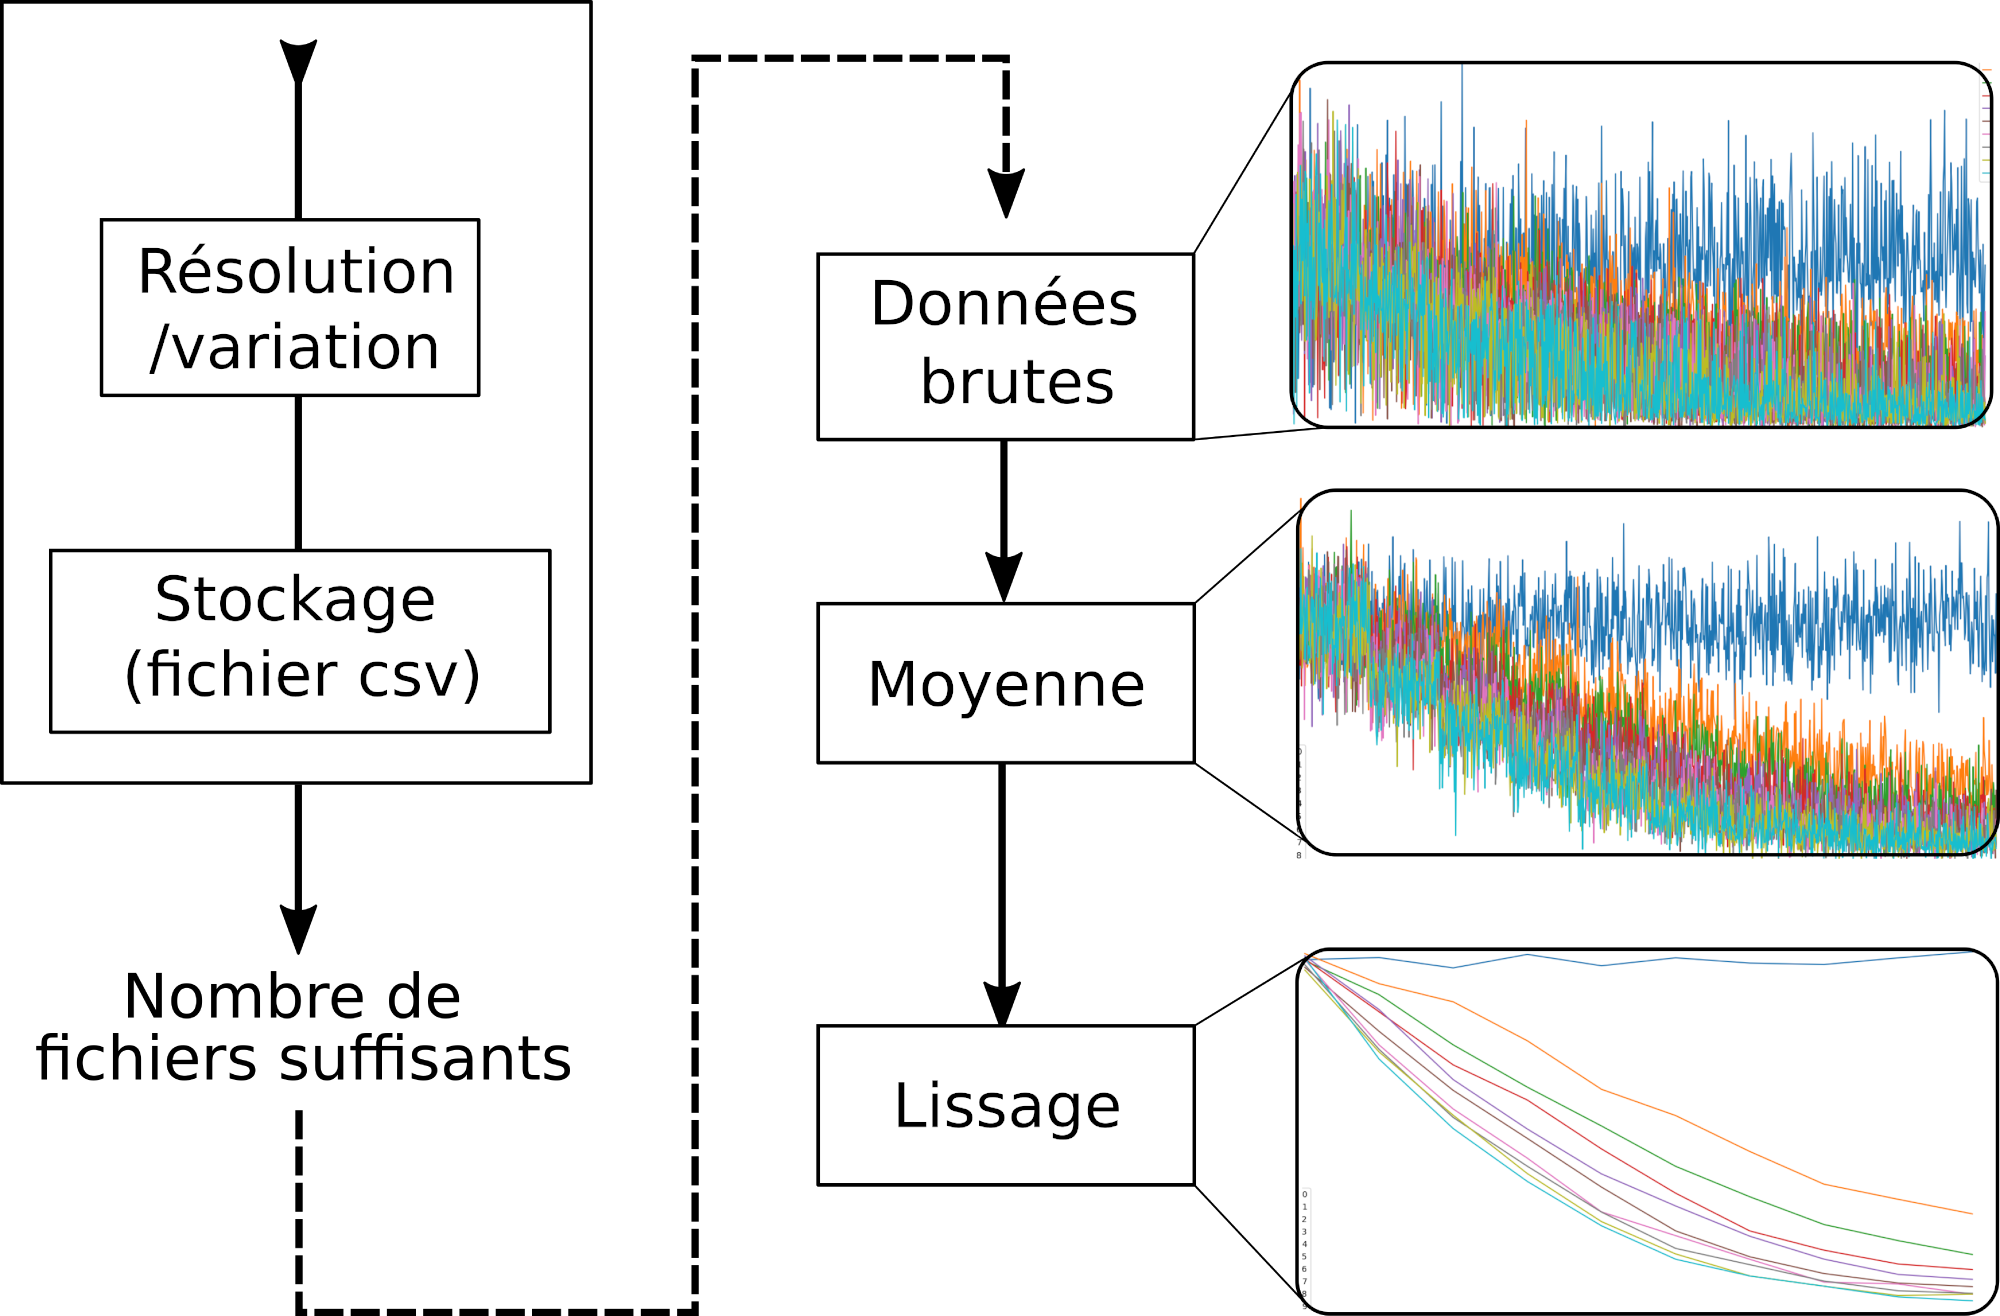
\includegraphics[width=10cm]{img/logigramme.png}
            \caption{Schéma du traitement des données à la sortie de l'algorithme}
            \label{logi}
          \end{figure}


      \subsection{Taille de la population}
        L'exécution du programme pour la variation de la taille de la population retourne les graphiques des figures \ref{evo_pop_size_brut} et \ref{evo_pop_size_moy}.

        \begin{figure}[h]
          \centering
          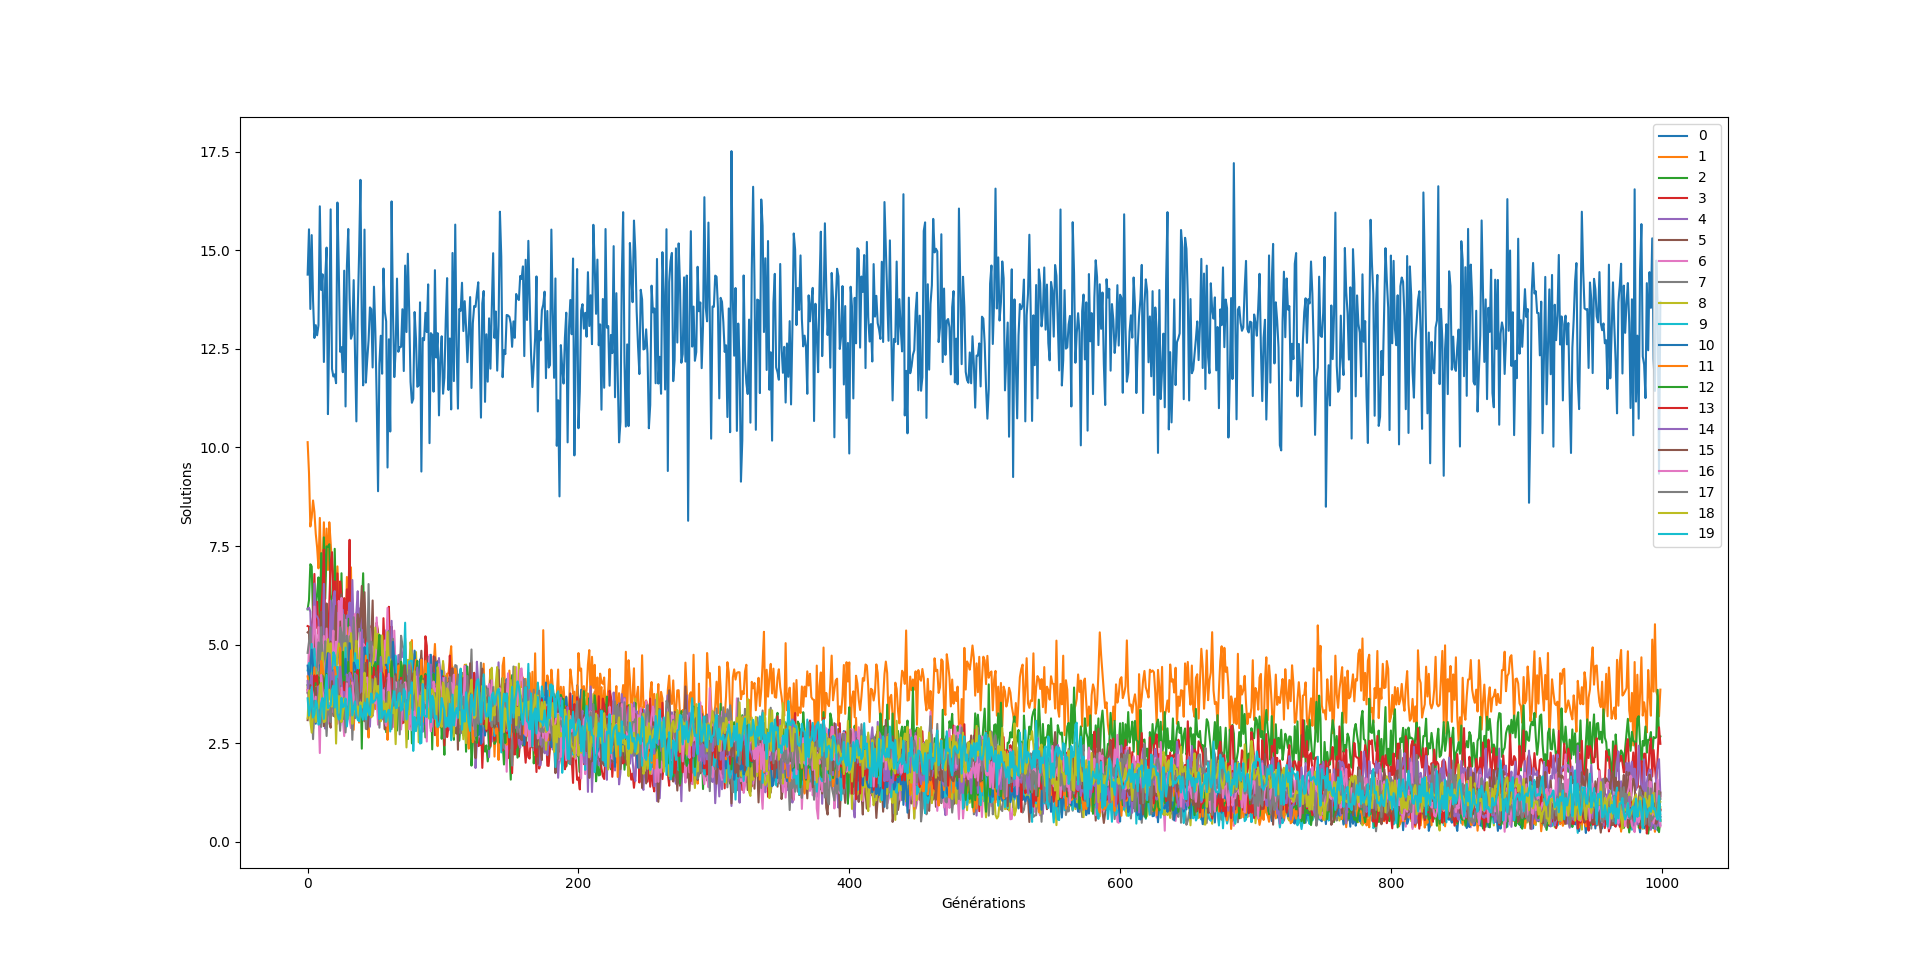
\includegraphics[width=18cm]{img/evo_pop_size_brut.png}
          \caption{Représentation de la solution au cours des générations - Variation de la taille de la population sur [0,2000] avec un pas de 100 - Autre paramètres : $P_{mutation} = 0.5$,$P_{crossover} = 0.5$}
          \label{evo_pop_size_brut}
        \end{figure}

        \begin{figure}[!]
          \centering
          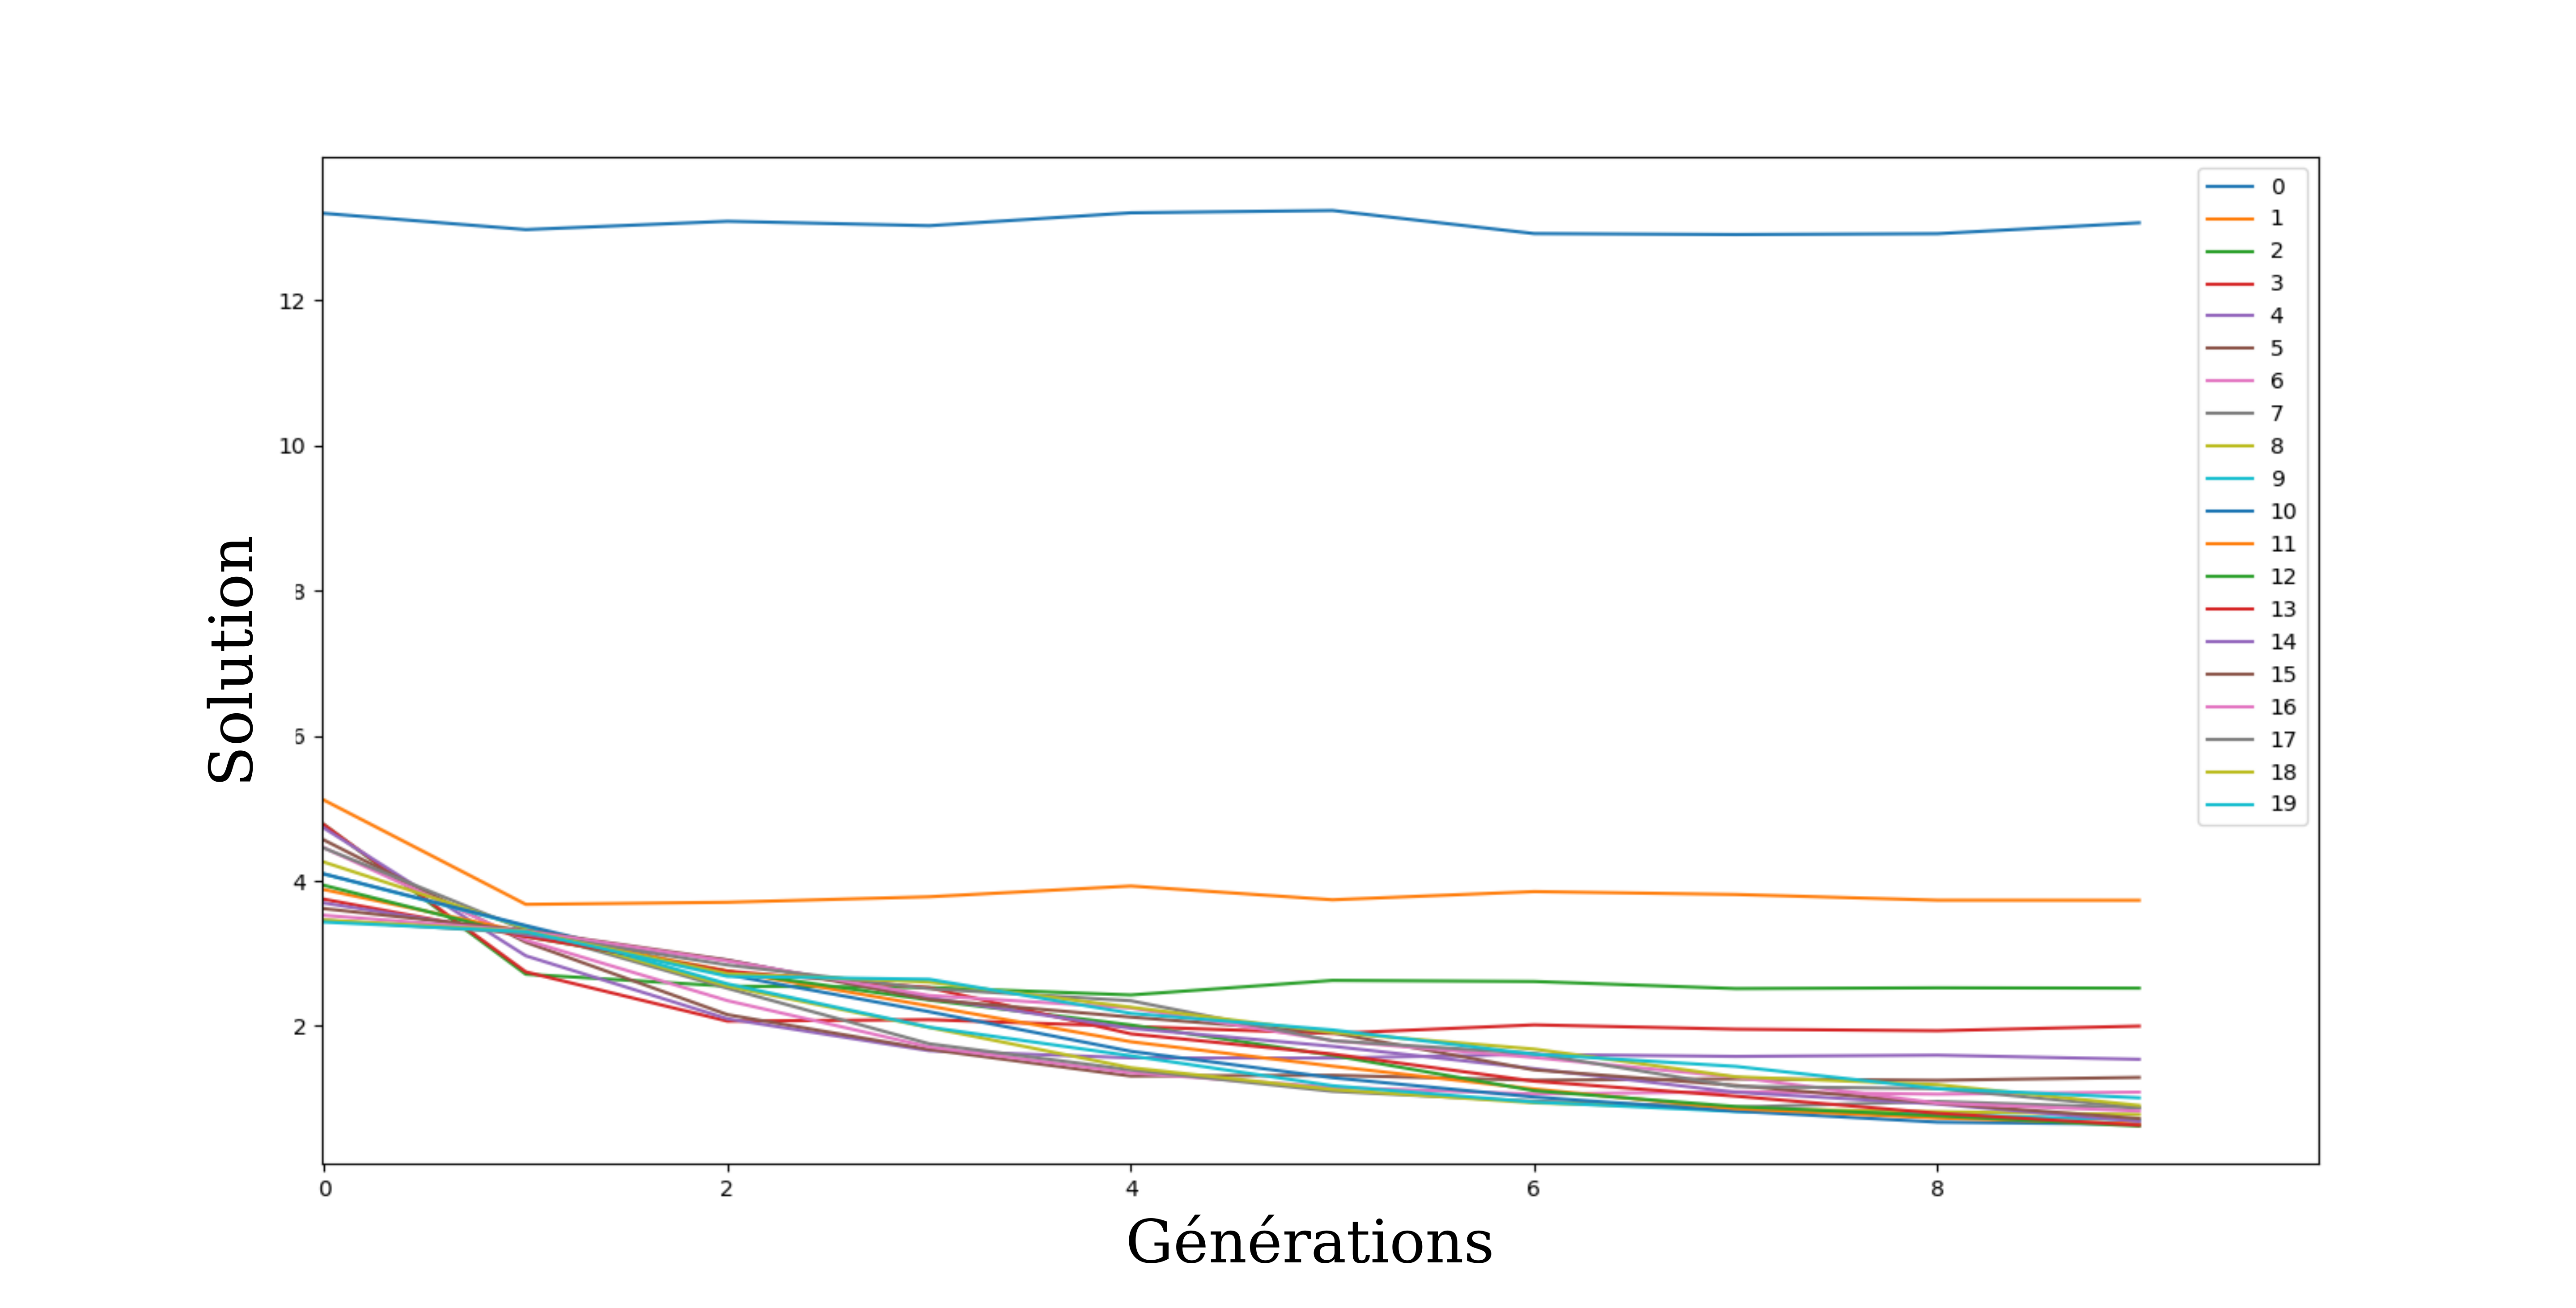
\includegraphics[width=18cm]{img/evo_pop_size_moy.png}
          \caption{Représentation "lissée" de la figure \ref{evo_pop_size_brut}}
          \label{evo_pop_size_moy}
        \end{figure}
        Le premier graphique (\ref{evo_pop_size_brut}) représente les données moyennes des fichiers (sans lissage), or bien que plus réaliste, cette représentation ne permet pas de tirer une conclusion quant à l'influence de ce paramètre sur l'algorithme. Afin d'éclaircir la figure on ramène un ensemble de points à une valeur moyenne de ces derniers (lissage), on obtient alors la figure \ref{evo_pop_size_moy} qui est beaucoup plus lisible. \\

        Dans un premier temps on remarque que la première courbe qui a été générée est largement au-dessus des autres. Cette courbe correspond à une taille de population de 10 alors que la suivante correspond à une population de 110. Lorsque l'on a une faible taille de population les solutions ont tendance à ne pas évoluer avec le nombre de générations. Cependant ce comportement s'améliore très rapidement avec l'augmentation progressive de ce dernier paramètre. Ceci explique le grand écart entre la population de 10 et la population de 110 individus.

        Si on met cette première courbe de côté, on remarque dans un second temps que lors des premières générations la convergence est semblable pour toutes les courbes, mais que plus on avance, plus les courbes s'écartent.
        \\ L'influence de la taille de la population se déduit donc très facilement : plus on a une population élevée, plus le résultat du programme va converger vers la solution du problème. On conclut donc que pour obtenir une solution de qualité il est nécessaire de prendre une grande population (au moins 2000 individus) et d'effectuer un nombre suffisant de générations.

      \subsection{Probabilité de croisement}

      \begin{figure}[h]
        \centering
        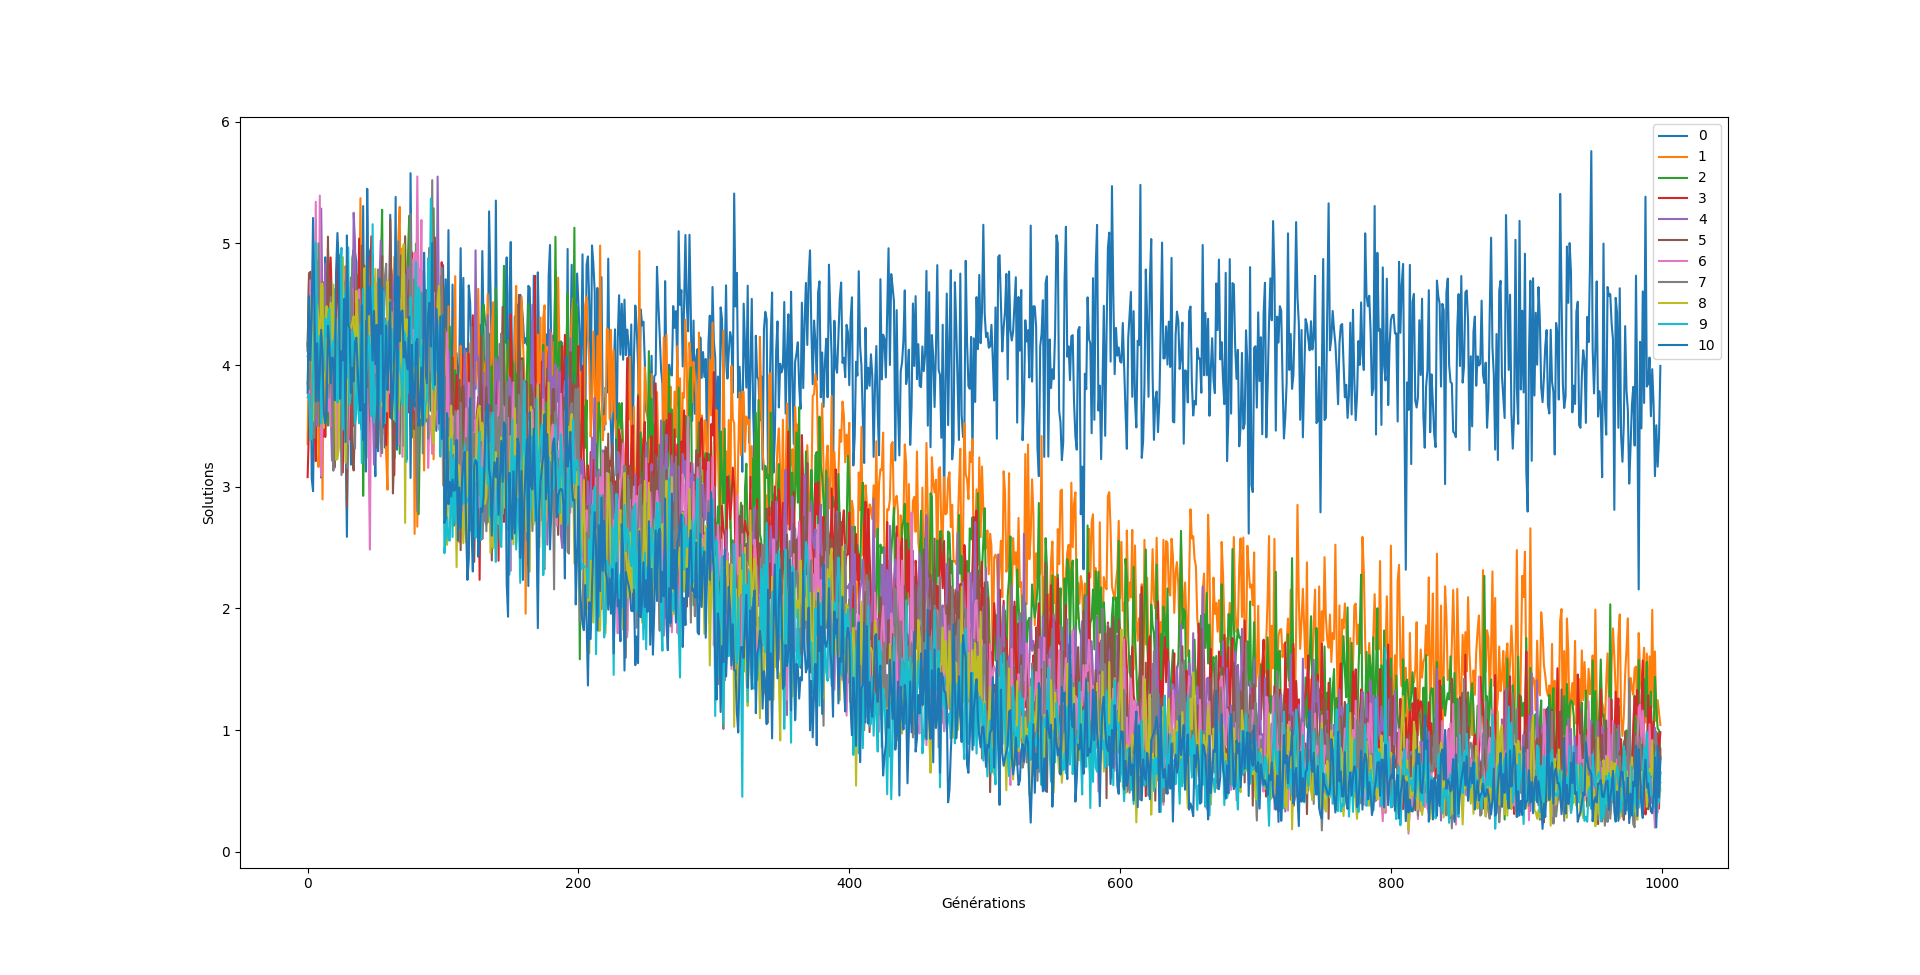
\includegraphics[width=15cm]{img/evo_crossover_brut.png}
        \caption{Représentation de la solution au cours des générations - Variation de la probabilité de croisement sur [0,1] avec un pas de 0.1 - Autre paramètres : $P_{mutation} = 0.5$, $population = 1000$}
        \label{evo_crossover_brut}
      \end{figure}

      \begin{figure}[!]
        \centering
        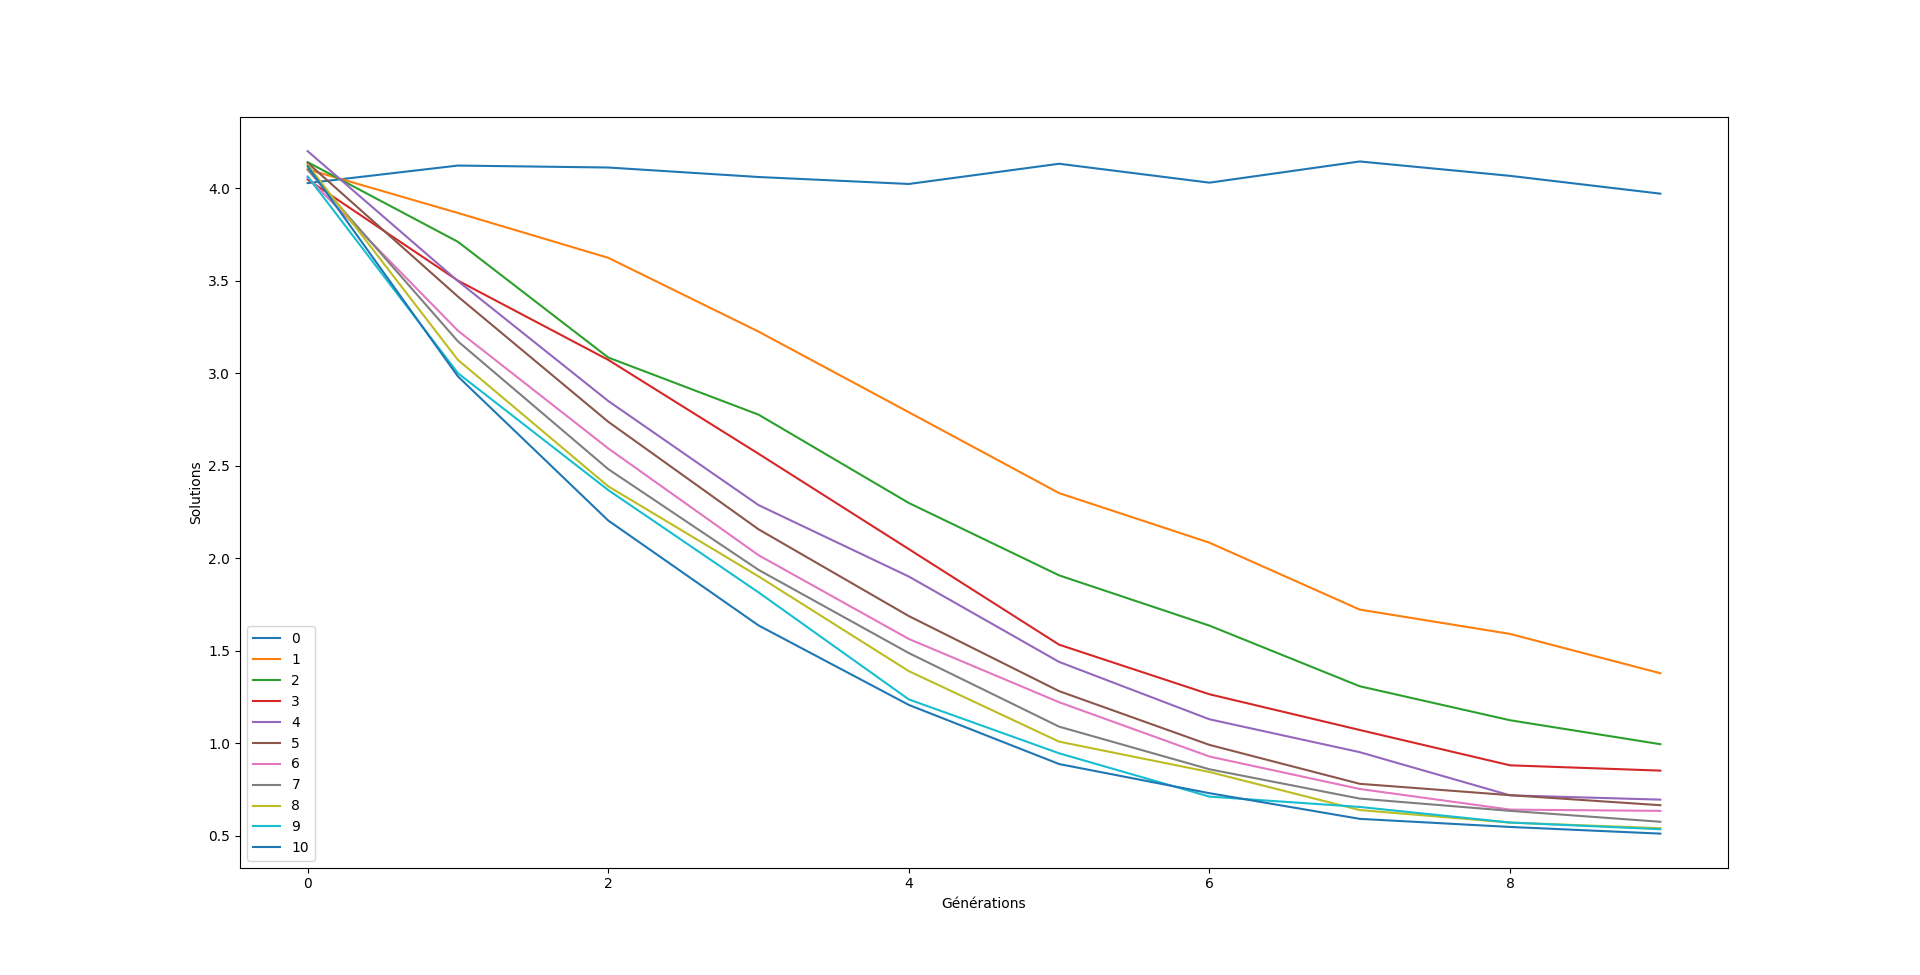
\includegraphics[width=15cm]{img/evo_crossover_moy.png}
        \caption{Représentation "lissée" de la figure \ref{evo_crossover_brut}}
        \label{evo_crossover_moy}
      \end{figure}

      Pour ce qui est de la variation de la probabilité de croisement, la première courbe correspond à une probabilité de 0. La solution n'évolue donc pas et reste au même niveau, peu importe le nombre de générations. Ensuite, plus la probabilité de croisement est haute plus la solution optimale est obtenue rapidement. Afin d'obtenir le meilleur résultat le plus rapidement possible, il faut alors choisir une probabilité de croisement très proche de 1 (en sachant que dans tous les cas la variation de ce paramètre n'a pas d'influence sur le temps de résolution).

      \subsection{Probabilité de mutation}

      \begin{figure}[h]
        \centering
        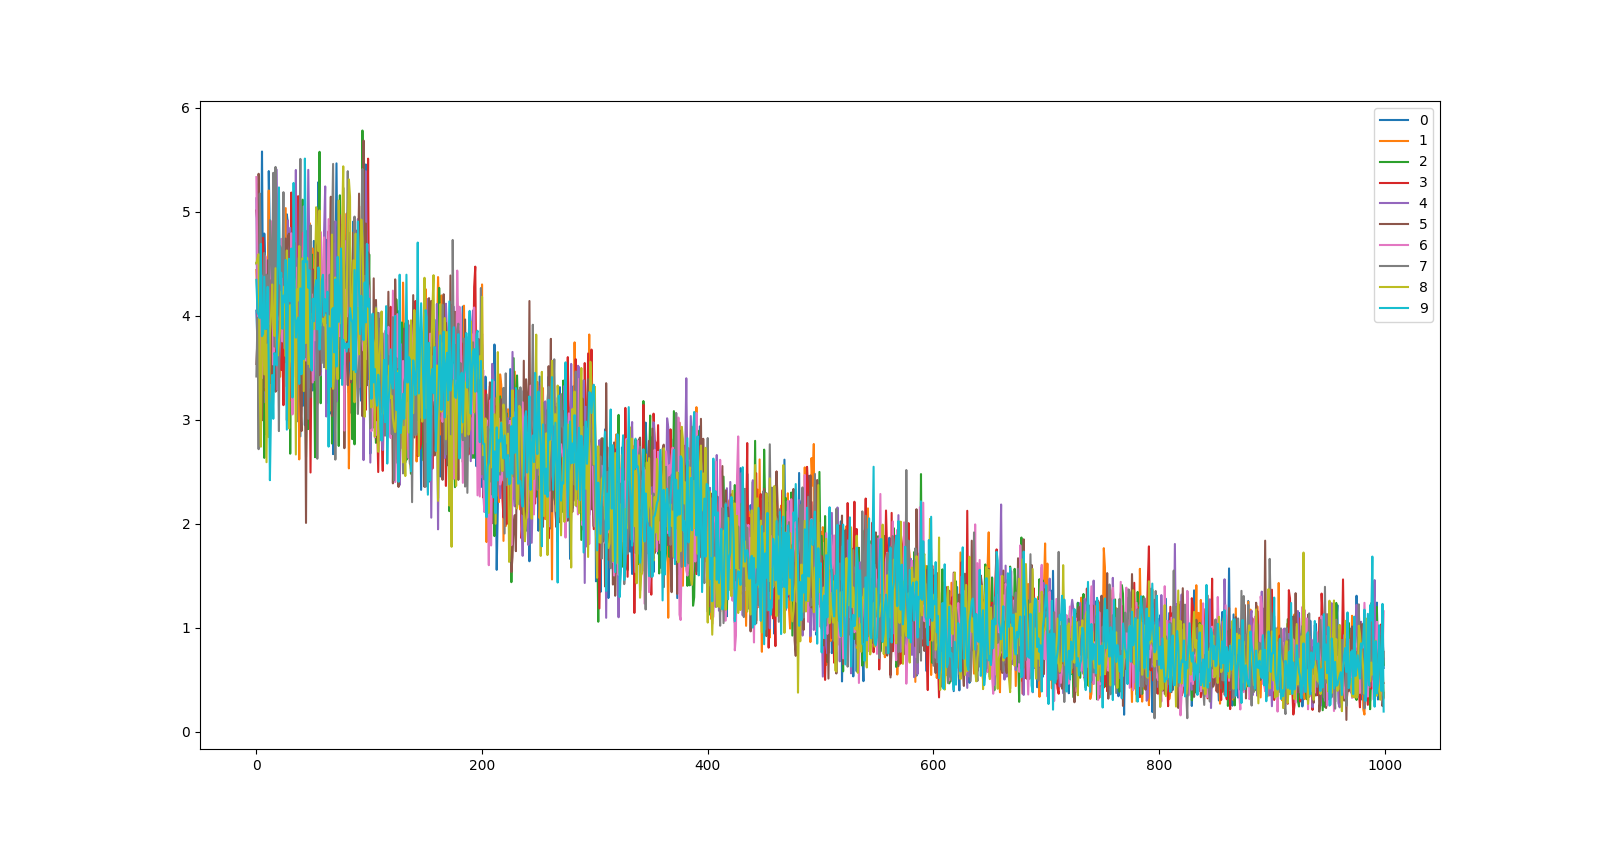
\includegraphics[width=17cm]{img/evo_mutation_brut.png}
        \caption{Représentation de la solution au cours des générations - Variation de la taille de la population sur [10,2000] avec un pas de 10 - Autre paramètres : $population = 1000$, $P_{crossover} = 0.5$}
        \label{evo_mutation_brut}
      \end{figure}

      \begin{figure}[!]
        \centering
        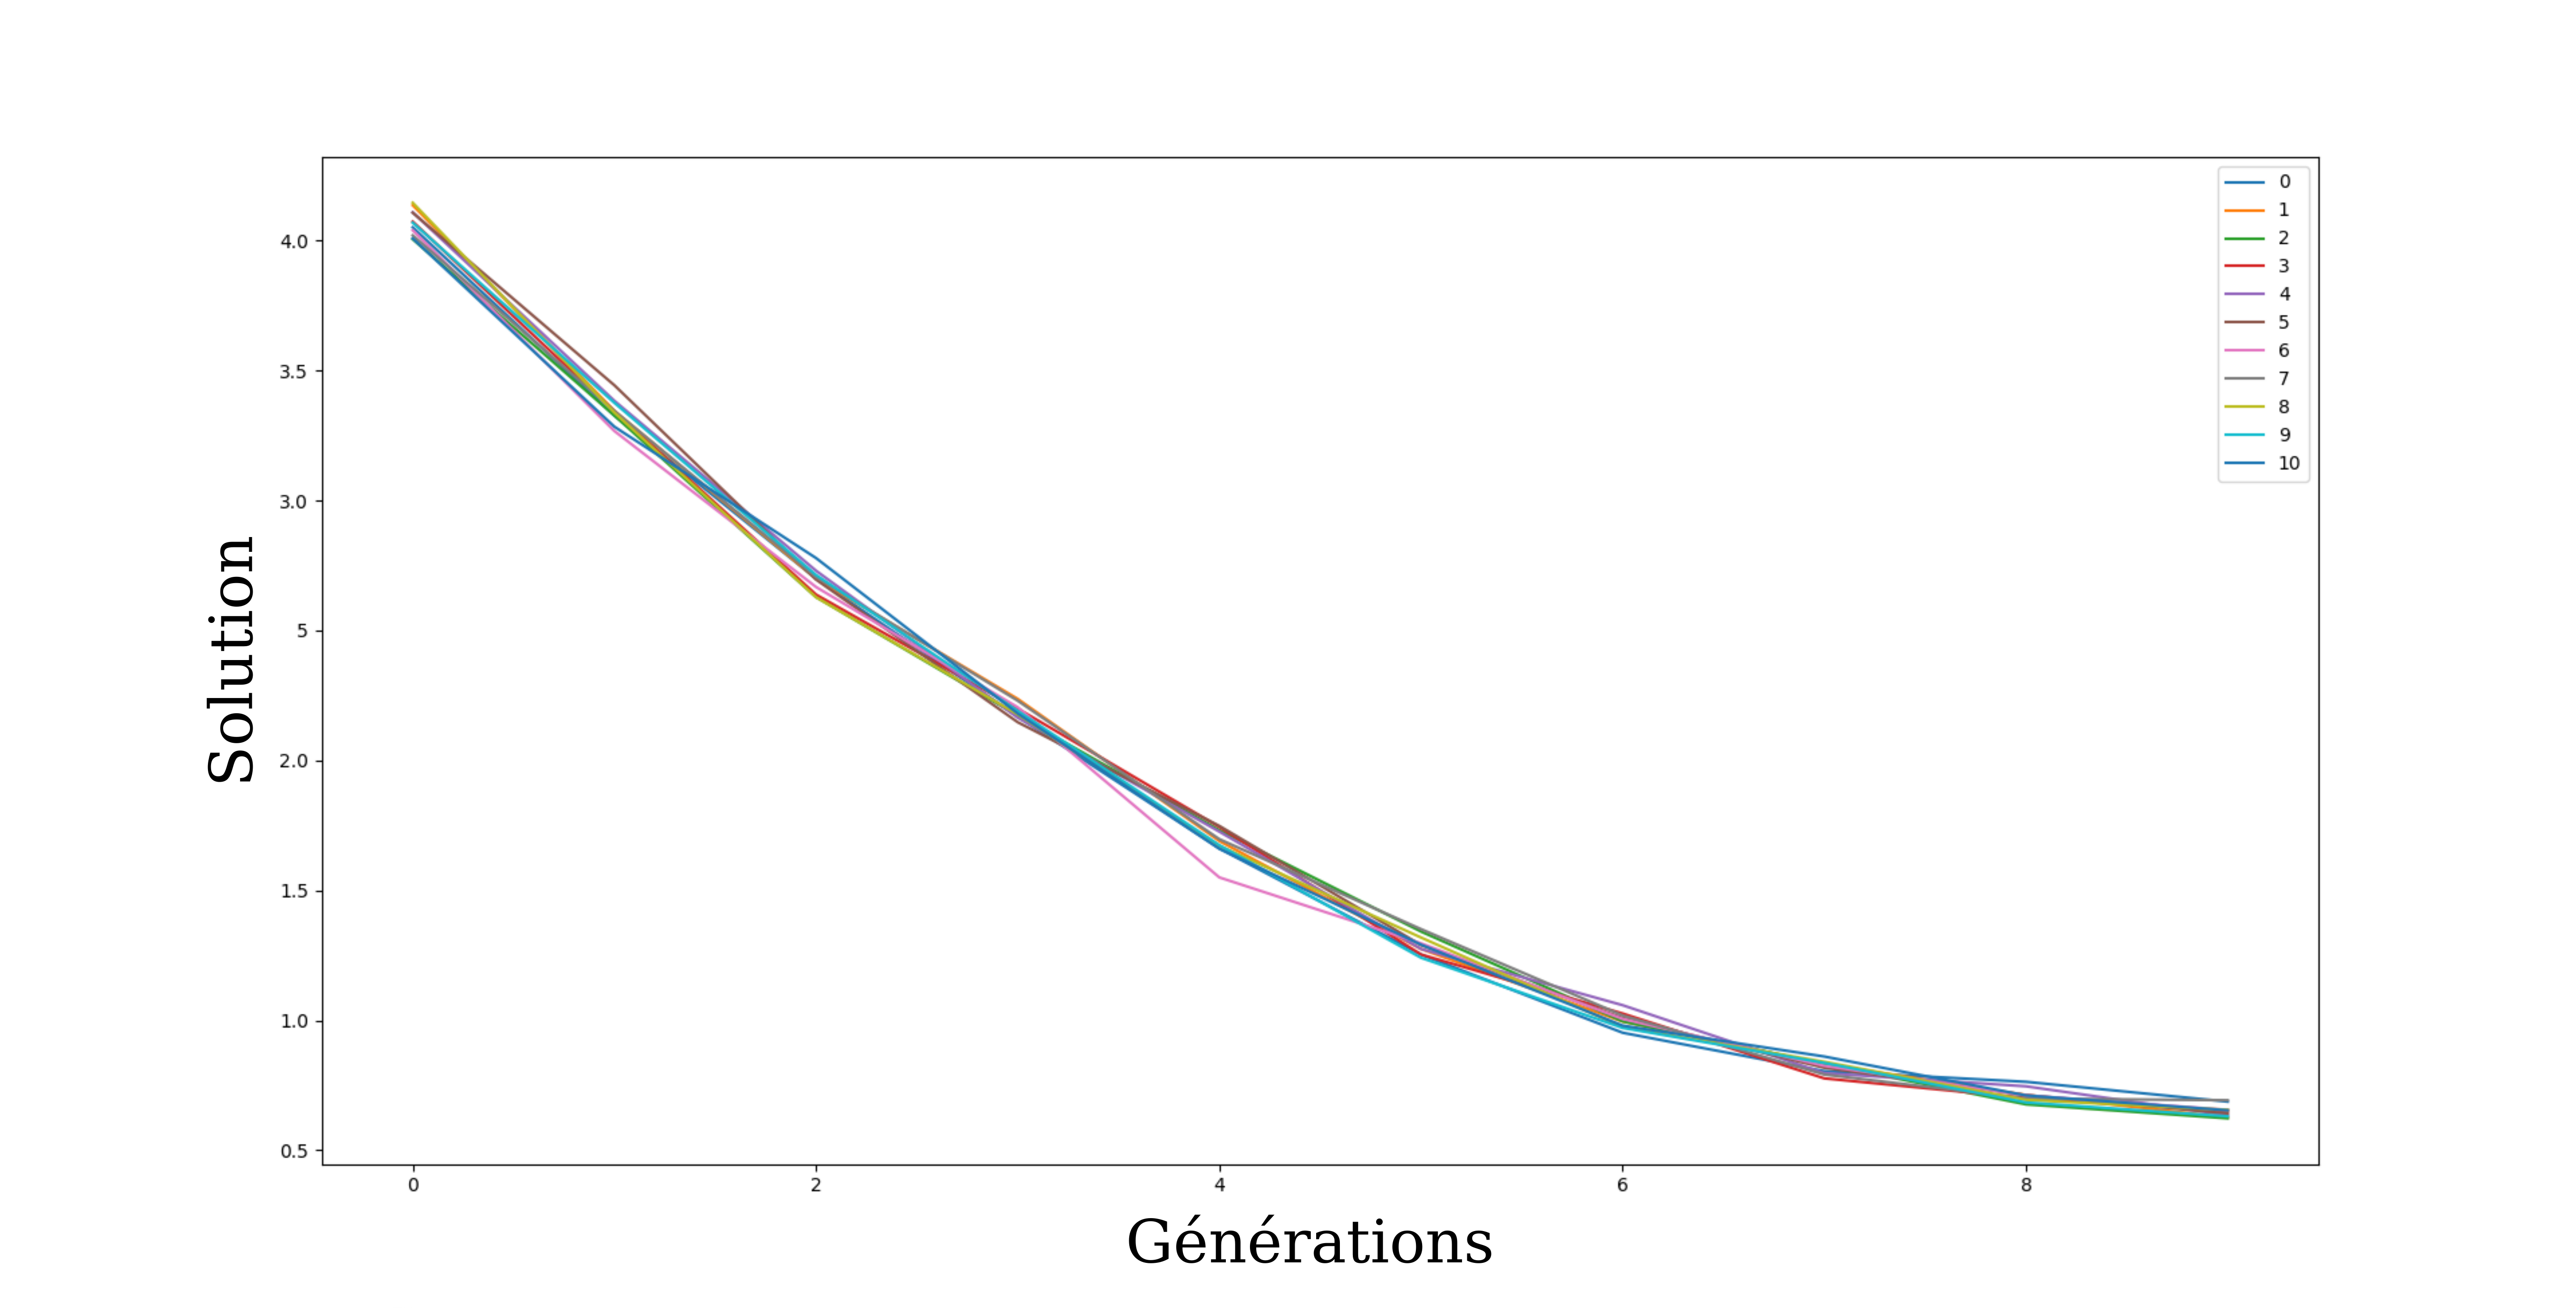
\includegraphics[width=17cm]{img/evo_mutation_moy.png}
        \caption{Représentation "lissée" de la figure \ref{evo_mutation_brut}}
        \label{evo_mutation_moy}
      \end{figure}

      Nous ne voyons ici aucune différence entre les courbes. La probabilité de mutation ne semble pas influer l'efficacité de la résolution. La mutation sert principalement à éviter de se coincer dans un minimum local en rajoutant de l'aléatoire dans les individus. Le fait qu'ici ce paramètre n'ait aucune influence peut s'expliquer par le fait que le problème est trop simple, la variation due à la probabilité de mutation est donc invisible pour nous.



  \chapter{Optimisation à objectifs multiples}
    \section{Algorithme - NSGAII}
    L'algorithme d'optimisation NSGAII (Non dominated sorting genetic algorithm 2) est un algorithme connu et utilisé à l'échelle mondiale pour sa fiabilité et ses performances. Ce type d'algorithmes diffère du premier par le nombre d'objectifs qu'il peut prendre en paramètre. Quand bien le premier algorithme ne pouvait chercher une solution que sur un problème mono-objectif, l'algorithme NSGA-II peut prendre plusieurs objectifs en paramètre. Cette différence entraine le changement de la nature des solutions, on parle alors de \emph{front de Pareto. (Ou d'optimum de Pareto)}\\

    \begin{figure}[h]
      \begin{minipage}[c]{.46\linewidth}
          \centering
          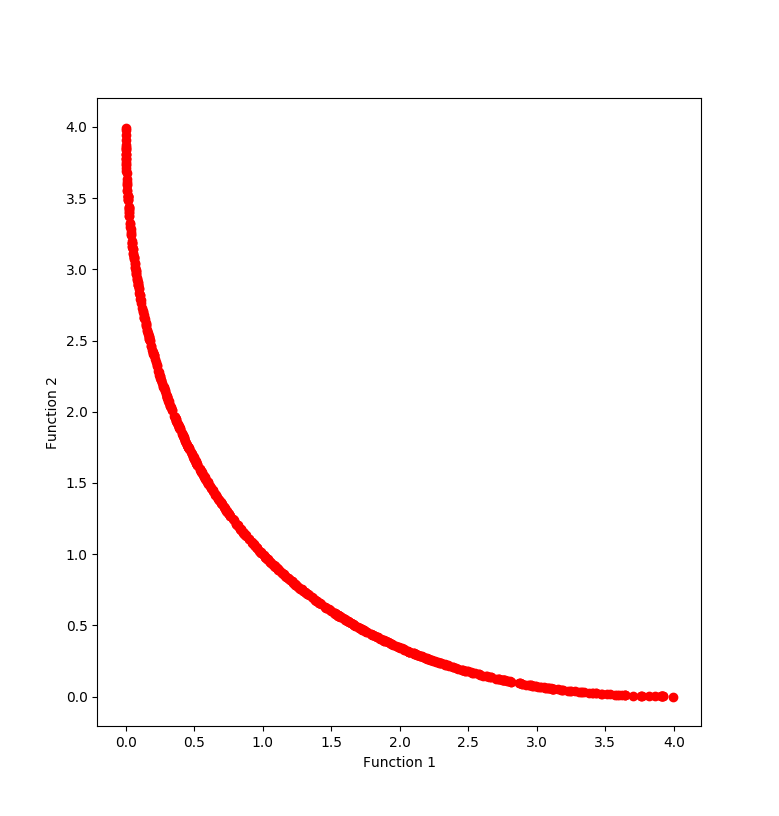
\includegraphics[width=6cm]{img/4,1,1_Pareto_uni.png}
          \caption{Front de Pareto du problème Schaffer N\degre1 \cite{wiki5} (bi-objectif)}
          \label{sch}
      \end{minipage}
      \hfill%
      \begin{minipage}[c]{.46\linewidth}
          \centering
          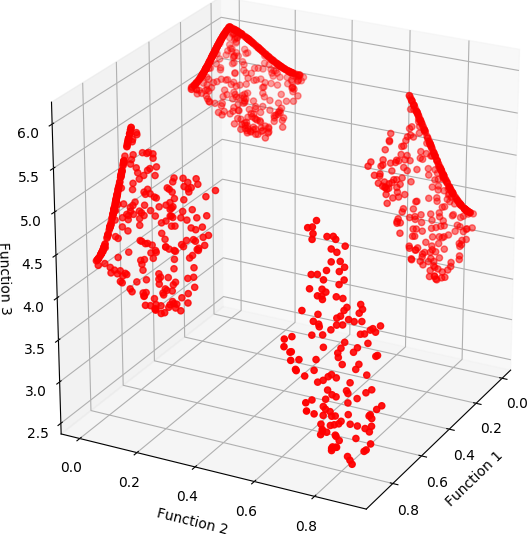
\includegraphics[width=6cm]{img/4,1,1_Pareto.png}
          \caption{Front de Pareto du problème DTLZ7 (tri-objectif)}
      \end{minipage}
    \end{figure}

    Le front de Pareto est une représentation graphique (figure \ref{sch}) de l'affirmation suivante :
    \begin{quotation}
      Il n'est pas possible d'améliorer la qualité de solution d'un objectif sans faire baisser celles des autres.
    \end{quotation}

    \emph{Remarque : Le front de Pareto ne donne pas directement les solutions du problème, car il s'agit de la représentation des images des solutions. Le but ici est de choisir un point sur le front de Pareto et d'aller chercher ensuite son(es) antécédent(s) pour chaque objectif.}

    \begin{quotation}
      Exemple : Dans le cas d'un problème bi-objectif unidimentionnel, pour un point $(a,b)$ sur le front de Pareto, la solution du problème est le doublet $(x,y)$ tel que $f(x)=a$ et $g(y)=b$.
    \end{quotation}



      \subsection{Principe}
      \begin{wrapfigure}{r}{7cm}
        \centering
        \includegraphics[width=6cm]{img/Pareto_domine.png}
        \caption{Front de Pareto - individus dominés/non dominés}
        \label{non_domine}
      \end{wrapfigure}
      L'algorithme NSGA-II reprend le principe de l'algorithme présenté dans la première partie, mais comporte quelques caractéristiques supplémentaires.


      \begin{description}
        \item [Approche élitiste] L'algorithme sauvegarde les meilleures solutions des générations précédentes (préservation de la diversité)
        \item [Non domination] L'algorithme trie les individus selon un ordre croissant de non-domination (Voir figure \ref{non_domine})
        \item [Croisement linéaire] Contrairement au croisement à n points du premier algorithme, les portions caractéristiques de chaque individu sont échangées aléatoirement et non par segment.
        \item [Mutation personnalisée] L'algorithme propose de choisir la méthode de mutation à utiliser \cite{wiki6}. Dans notre cas, la mutation gaussienne est utilisée du fait de sa popularité auprès des utilisateurs de la bibliothèque Inspyred \cite{inspyred}.
      \end{description}

      \begin{figure}[h]
        \centering
        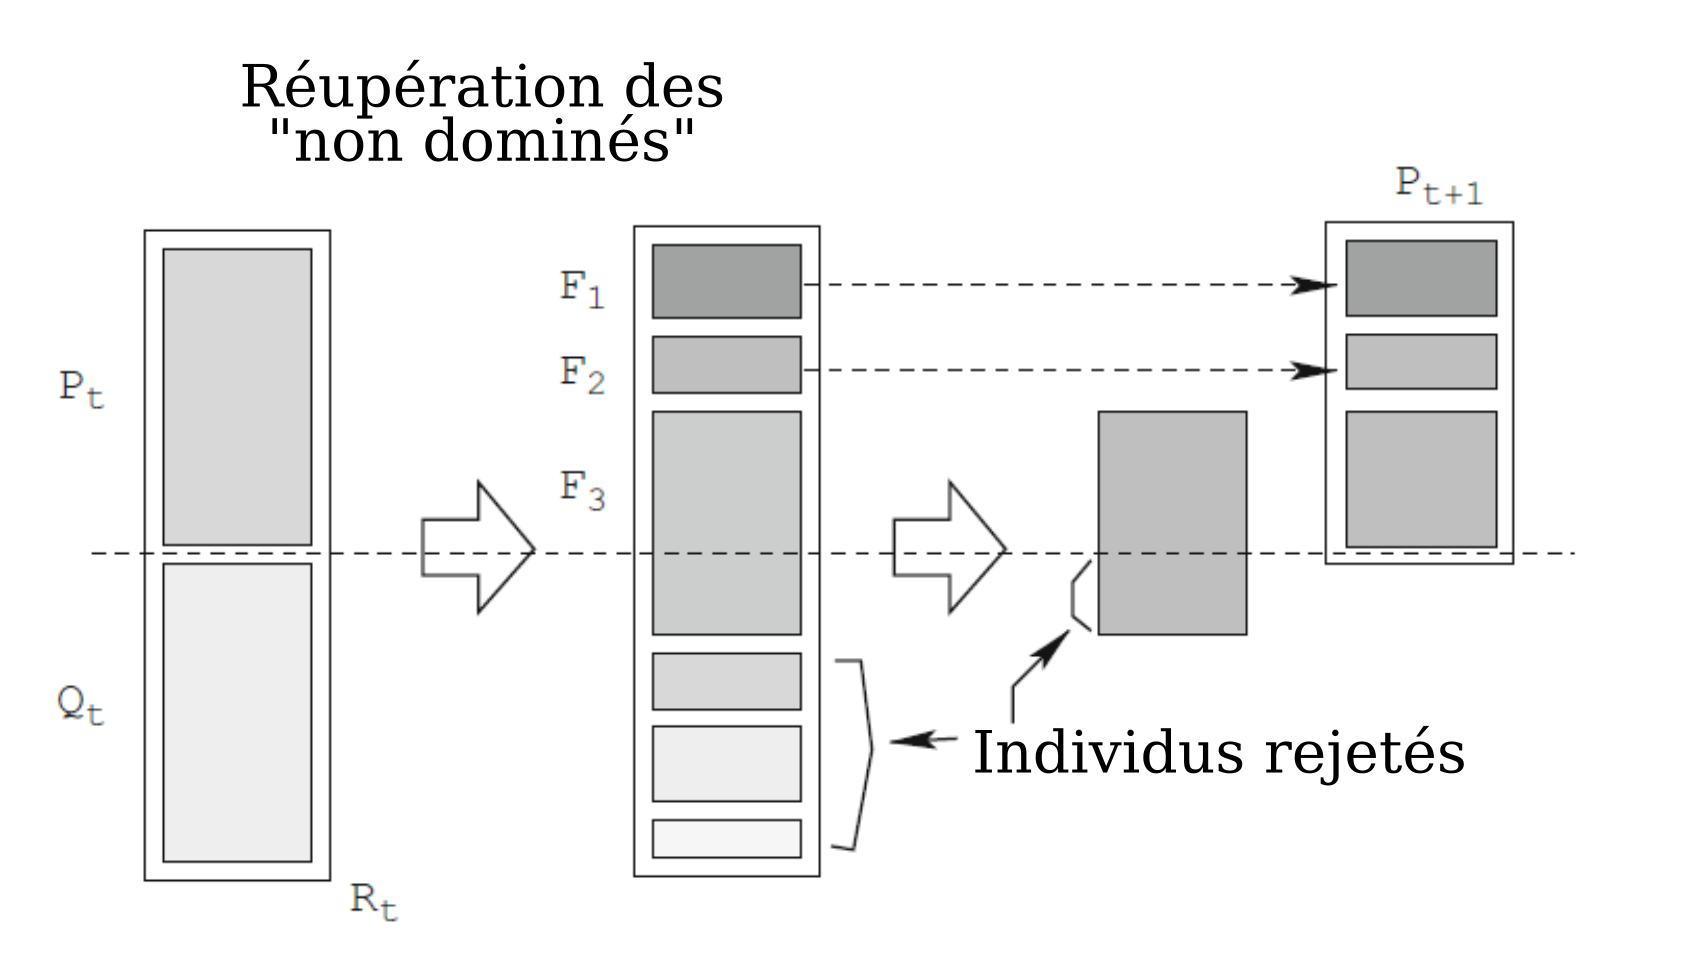
\includegraphics[width=12cm]{img/sch_nsga2.png}
        \caption{Schéma de fonctionnement NSGA2}
        \label{sch_nsga2}
      \end{figure}

      \emph{La figure \ref{sch_nsga2} schématise le fonctionnement de l'algorithme}
      \begin{enumerate}
        \item Initialement, une population d'individus est formée aléatoirement puis est triée sur le principe de non-domination.
        \item Les individus résultants forment la population $P_{t}$ (figure \ref{sch_nsga2}) qui se dédouble en $Q_{t}$ par croisement et mutation.
        \item L'ensemble $R_{t}$ est ensuite trié toujours sur le principe de non-domination, puis divisé en deux (en rejetant les individus à l'indice de domination trop élevé).
        \item On se retrouve alors avec une population $P_{t+1}$ prête à retourner à l'étape 2.
      \end{enumerate}


    \section{Méthode de comparaison des résultats}
      \begin{wrapfigure}{r}{5cm}
        \centering
        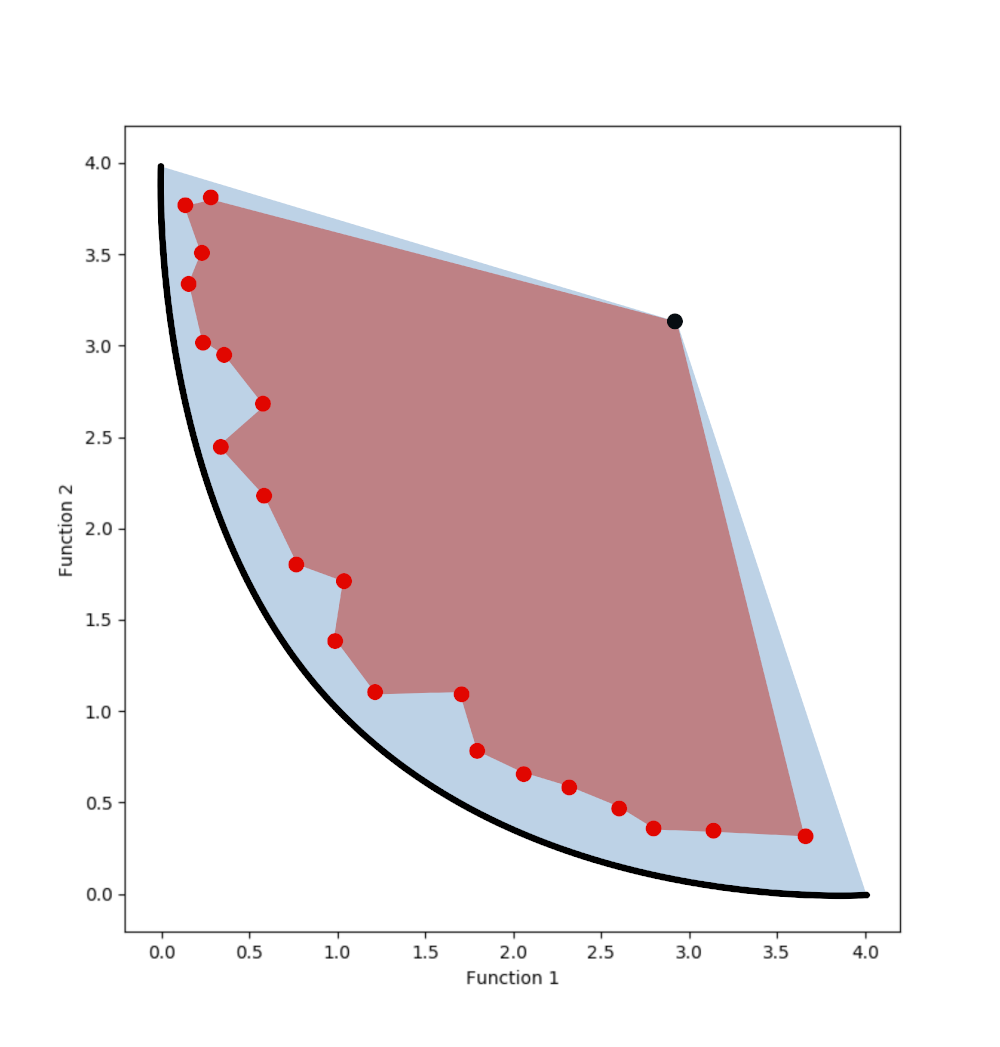
\includegraphics[width=6cm]{img/hypervolume.png}
        \caption{Représentation de la méthode de calcul du l'hypervolume}
        \label{hypervolume}
      \end{wrapfigure}
      Comme nous l'avons vu en abordant la notion de front de Pareto, le type solution recherché dans le cadre d'une optimisation multiobjectif n'est pas le même que dans un problème mono-objectif. Lorsque l'on cherchait une et une seule valeur avec le premier algorithme, l'objectif est ici de minimiser plusieurs fonctions à la fois. Notre but final étant d'étudier l'influence du paramétrage il est essentiel de pouvoir caractériser l'évolution de chaque algorithme. \\
      Dans le cas présent, pour un problème multiobjectif il est possible d'étudier l'évolution du front de Pareto géométriquement en calculant l'aire, le volume ou plus généralement l'hypervolume de ce dernier.
      Prenons un exemple simple dans un problème ou l'on cherche à minimiser deux fonctions (Figure \ref{hypervolume}). La courbe noire représente le front de Pareto de référence et les points rouges un front trouvé à l'aide de l'algorithme NSGAII (peu d'individus et peu de générations). On pose un point sur le plan et on calcule les aires des fronts noir et rouge en tenant compte du point A. On obtient alors deux valeurs réelles comparables qui permettent d'étudier la convergence du front de Pareto au cours des générations (plus les valeurs sont semblables, plus la qualité du Pareto est bonne).
    \section{Influence du paramétrage}
      \subsection{Protocole}

      De la même façon qu'avec le premier algorithme on cherche à observer l'influence du paramétrage sur la qualité de la solution. Les seules différences notables avec la première observation sont :
      \begin{itemize}
        \item On change de type de problème (multiobjectifs) :
        $$
        \forall x \in [-10,10],
        \left\{
          \begin{array}{ll}
             f_1(x) = x^2 \\
             f_2(x) = (x-2)^2
          \end{array}
        \right.
        $$
        \item Les courbes représentent désormais l'évolution de l'hypervolume et non plus l'évolution de la solution directement.
      \end{itemize}


      \subsection{Taille de la population}
      La taille de la population dans l'algorithme NSGA-II est un paramètre important car il fait varier de façon significative le temps de résolution du problème. Ainsi, pour une population d'individus supérieure à 500, le temps de résolution devient trop important pour exécuter notre programme de variation dans de bonnes conditions (nombre de générations élevé). Dans cette partie on se contente donc d'une population allant de 10 individus à 150 avec un pas de 10 et de 50 générations maximum. On obtient alors la figure \ref{sch_pop_size_moy} qui donne la figure \ref{sch_pop_size_liss} (Lissage).

      \begin{figure}[h]
        \centering
        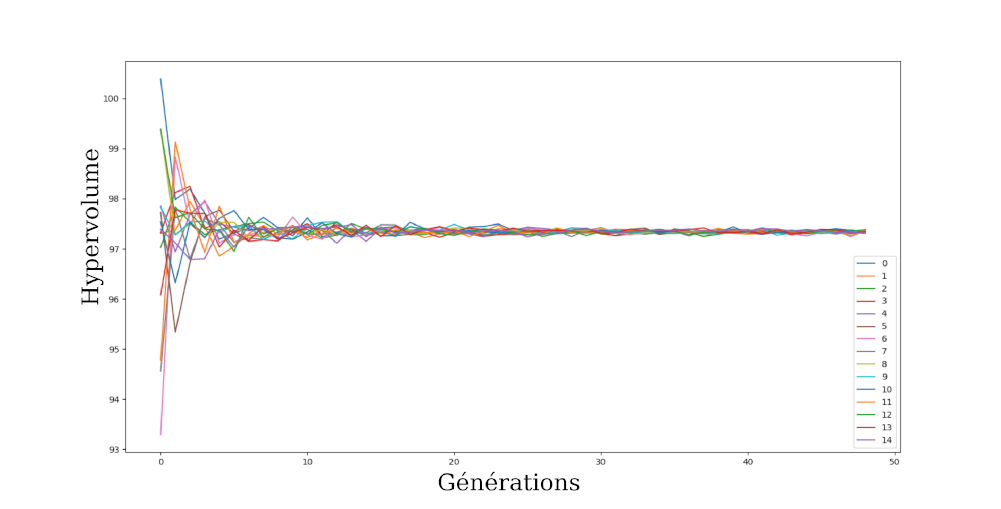
\includegraphics[width=18cm]{img/pop_size_sch_moy.png}
        \caption{Représentation de l'hypervolume au cours des générations - Variation de la taille de la population sur [10,150] avec un pas de 10 - Autre paramètres : $P_{mutation} = 0.5$,$P_{crossover} = 0.5$}
        \label{sch_pop_size_moy}
      \end{figure}

      \begin{figure}[!]
        \centering
        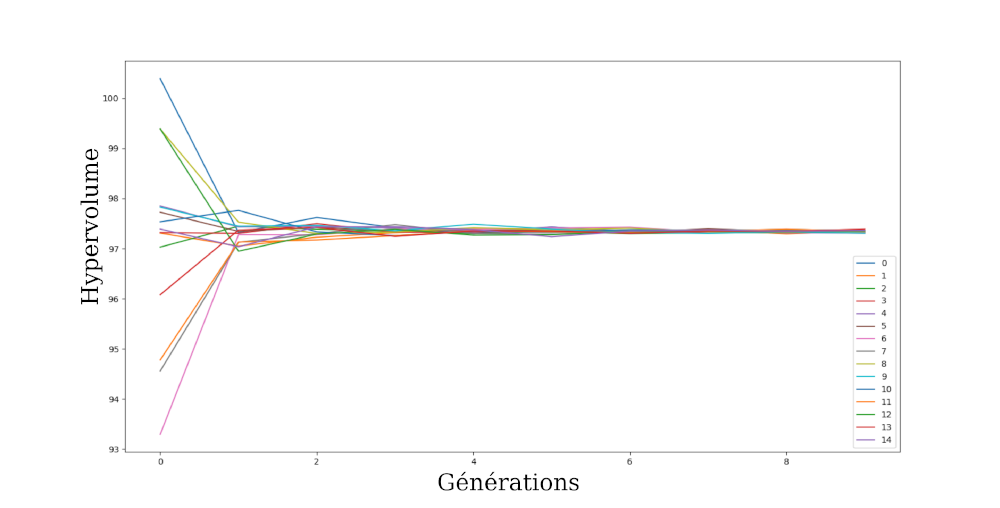
\includegraphics[width=18cm]{img/pop_size_sch_liss.png}
        \caption{Représentation "lissée" de la figure \ref{sch_pop_size_moy}}
        \label{sch_pop_size_liss}
      \end{figure}


      Contrairement aux figures extraites du premier algorithme, on voit bien qu'ici la variation de ce paramètre influence bien moins la qualité de la solution, voire même ne l'influence pas du tout. En effet toutes les courbes convergent très rapidement et de la même façon vers la valeur de référence du problème, on ne distingue pas différence notable entre la courbe correspondant à 10 individus et celle correspondante à 150 individus.

      On se doute que si nous avons la possibilité de changer la taille de la population c'est que ce paramètre influence forcément le résultat de l'algorithme. Selon nous le constat que nous faisons ci-dessus peut s'expliquer de deux façons :
      \begin{enumerate}
        \item Nous exécutons l'algorithme sur un problème trop simple, ainsi la solution optimale est atteinte très rapidement et gomme au passage toute la partie de convergence des courbes qui nous intéresse.
        \item Nous faisons varier la taille de la population de façon trop peu importante pour observer une différence entre chaque courbe.
      \end{enumerate}

      Pour répondre à ces questions on tente une résolution du problème DTLZ7 nettement plus complexe :

[DTLZ]
      À cause d'un temps important de résolution, on exécute le programme sur seulement une dizaine de générations et une population allant de 10 à 400 avec un pas de 10.
      On obtient le résultat de la figure \ref{DTLZ7_pop}.
      \begin{figure}[h]
        \centering
        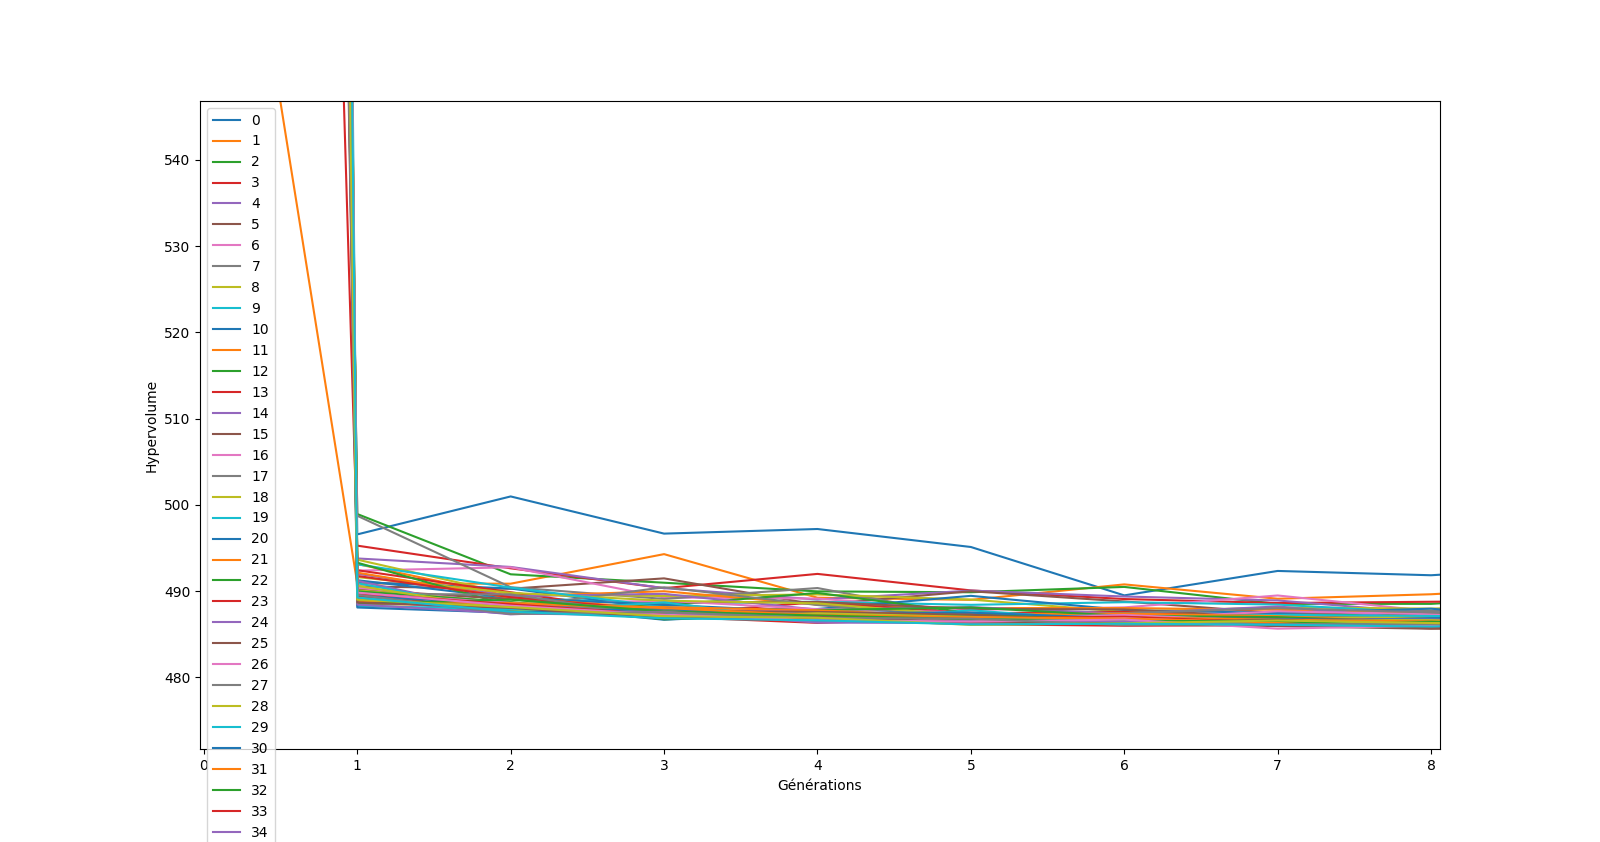
\includegraphics[width=15cm]{img/DTLZ7_pop.png}
        \caption{Représentation de l'hypervolume au cours des générations - Variation de la taille de la population sur [10,400] avec un pas de 10 - Autre paramètres : $P_{mutation} = 0.5$,$P_{crossover} = 0.5$}
        \label{DTLZ7_pop}
      \end{figure}

      On observe alors que contrairement au problème SCH, la population influence ici le résultat : plus elle est importante, plus la valeur de référence de l'hypervolume est atteinte rapidemmnt. En revanche, à cause du nombre de génération très limité (lié à la capacité de calcul de nos ordinateurs), on ne sait pas ce qu'il advient de ces courbes après 10 générations. Il est par exemple possible que comme avec le premier algorithme les courbes correspondantes à une population faible semblent tendre vers une valeur qui est supérieure à la valeur de référence.
      Dans tous les cas, selon nos observations, afin d'obtenir un résultat convenable sur une période de temps relativement courte il est nécessaire de fournir à l'algorithme une population suffisament élevée d'au moins 100 à 200 individus.

      \subsection{Probabilité de croisement}
      \emph{Comme dans la partie précédente concernant la taille de la population il s'est avéré que le problème SCH était trop simple, on utilisera dans la suite de ce chapitre la fonction DTLZ7 (définie ci-dessus).}
      Comme nous l'avons expliqué dans le principe de l'algorithme NSGA-II, ce dernier utilise une méthode de croisement différente du premier algorithme : le croisement linéaire.
      Or bien que cette méthode de croisement est répandue, lors de la variation de probabilité de croisement (même pour un problème difficile comme DTLZ7) on n'observe pas de différence majeur entre toutes les courbes. Tout comme la variation de la population avec la fonction SCH, on peut faire des suppositions sur les raisons de cette stabilité :
      \begin{itemize}
        \item La difficulté sur problème n'est peut être toujours pas assez élevée.
        \item Le pas de variation de la probabilité de croisement est peut être trop grand pour observer la répartition des courbes sur le graphique.
      \end{itemize}

      \begin{figure}[h]
        \centering
        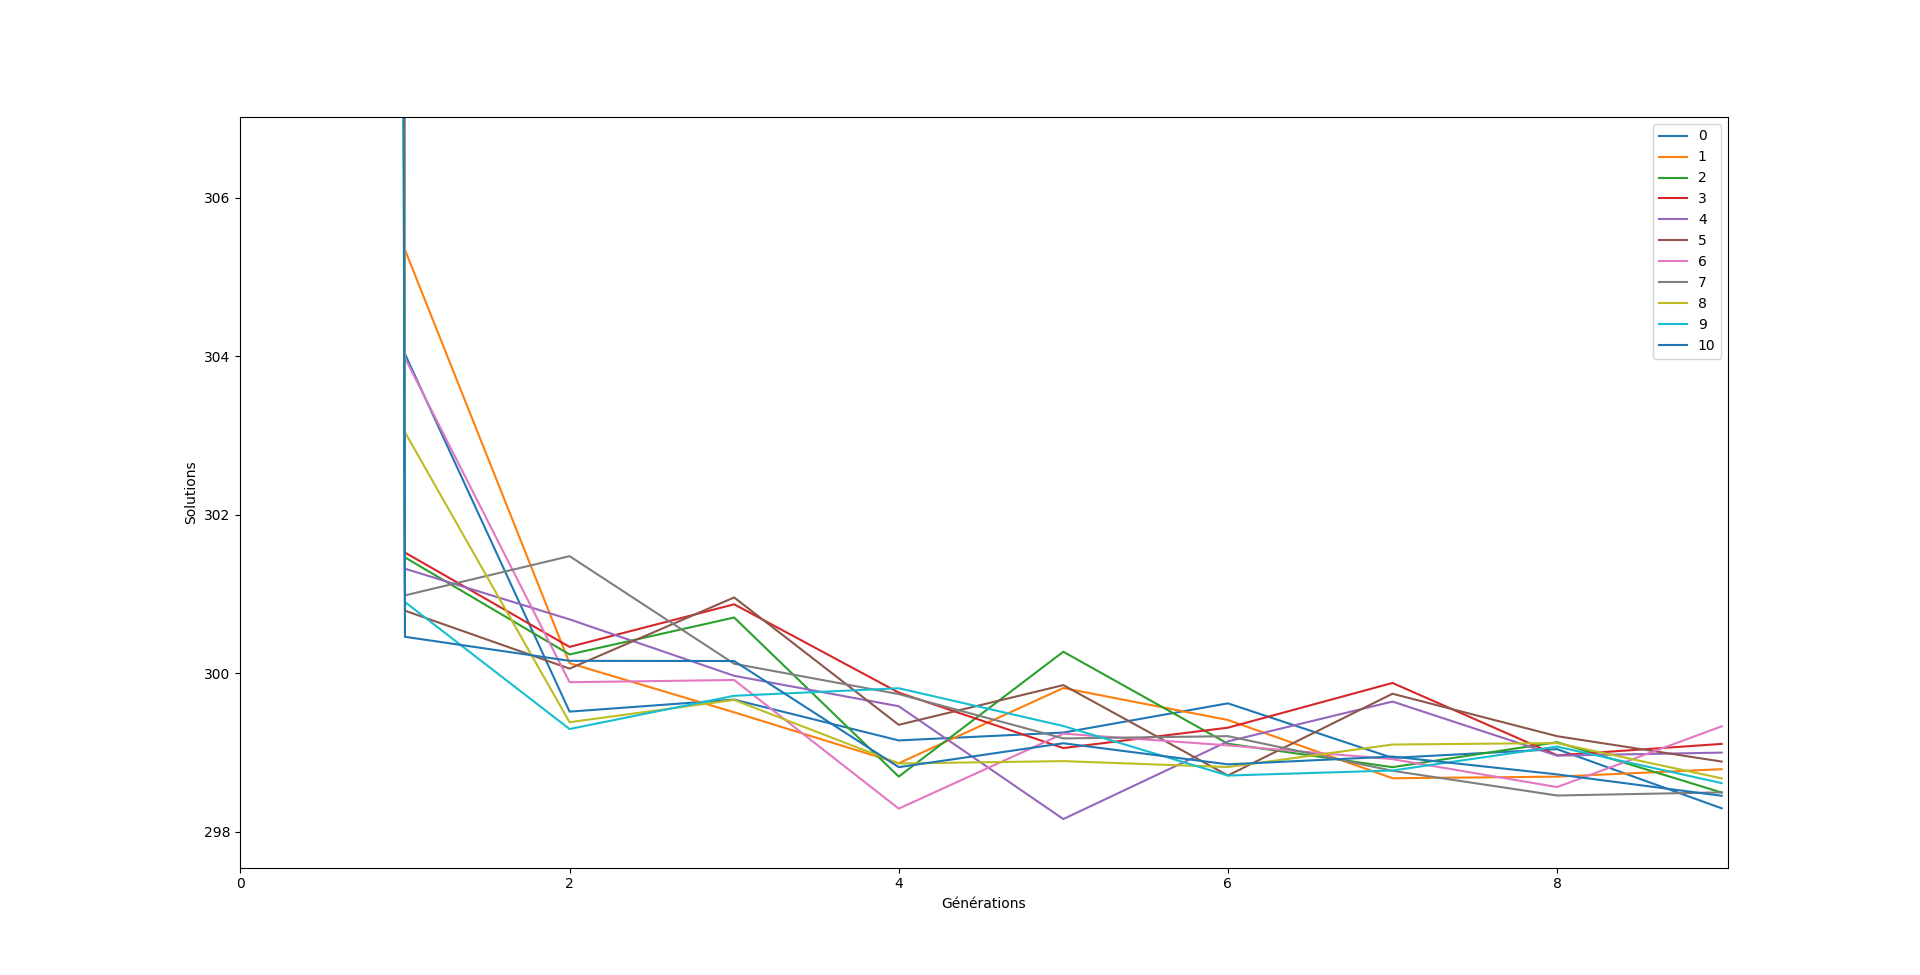
\includegraphics[width=15cm]{img/DTLZ7_crossover.png}
        \caption{Représentation de la solution au cours des générations - Variation de la taille de la population sur [10,2000] avec un pas de 10 - Autre paramètres : $population = 1000$,$P_{crossover} = 0.5$}
        \label{sch_crossover_moy}
      \end{figure}

      Enfin, la variation de la probabilité de muation nous donne la figure \ref{sch_mutation_moy}. On remarque que contrairement à toutes les figure précédentes, l'augmentation de la probabilté de mutation n'ameillore pas la convergence vers la solution de référence, mais que au contraire elle la dégrade. Et d'ailleur, si on reprend la définition de la mutation dans les cadre des algorithmes génétiques cela parrait logique. La mutation n'est pas là pour ameillorer la vitesse de convergence, mais plutot pour éviter à l'algorithme de tombrer dans un extremum local.
      Il faut donc adapter ce paramètre au problème que l'on essaye de résoudre :
      \begin{itemize}
        \item Si le problème possède beaucoup d'extremums locaux : on définit un probabilité de mutation élevée
        \item Sinon : on peut donner une valeur très faible à ce paramètre (voir même un valeur nulle)
      \end{itemize}

      \subsection{Probabilité de mutation}
      \begin{figure}[h]
        \centering
        \includegraphics[width=15cm]{img/DTLZ7_mutation.png}
        \caption{Représentation de la solution au cours des générations - Variation de la taille de la population sur [10,2000] avec un pas de 10 - Autre paramètres : $population = 1000$,$P_{crossover} = 0.5$}
        \label{sch_mutation_moy}
      \end{figure}



  \chapter{Conclusion}

  Nous avons pu voir au travers de deux algorithmes génétiques de natures différentes que leur paramétrage influence réellement les caractéristiques de leurs solutions. Ainsi, avec l'étude sur l'influence des paramètres que nous avons menée il est possible pour un utilisateur de choisir le bon paramétrage en fonction du résultat qu'il veut obtenir.
  Tout au long de ce projet, un élément est resté central et mériterait sans doute qu'on s'y intéresse de façon plus poussée : le temps. Car quand bien il est possible d'obtenir une solution de qualité sur une période de résolution longue, il est aussi possible d'obtenir un résultat sensiblement identique sur un laps de temps beaucoup plus court. Et c'est ici que le paramétrage prend toute son importance : un mauvais paramétrage donnera une solution au bout d'un moment, mais un bon la donnera beaucoup plus rapidement et avec une qualité bien supérieure.

  Dans ce projet nous nous sommes catonnés à deux d'algorithmes qui représentent les algorithmes "types" dans le monde de l'optimisation génétique, mais il est à noter qu'il existe des centaines d'algorithmes génétiques, tous plus ou moins puissants et qui s'adaptent à certains problèmes en particulier. On peut par exemple citer tous les algorithmes génétiques qui ont été développés pour résoudre le \emph{problème du voyageur de commerce \cite{wiki7}}. De la même façon, cette fois-ci dans le monde industriel, de nombreux algorithmes sont très utilisés pour résoudre des problèmes d'optimisation au coeur des entreprises ou des bureaux d'études (MOGA, NSGA-III, PESA, NPGA...etc \cite{diapo}).


   L'ensemble des programmes qui ont été utilisé pour réaliser ce projet sont soumis à la license \emph{GNU General Public License v3.0} et sont donc sont mis à disposition sur notre page GitHub : \\\\
   \url{https://github.com/Akashita/AG-USMB}


  \appendix

  \chapter{Fiche synoptique}

  \section{Généralités}
  \begin{description}
    \item[Titre du sujet] Optimisation par algorithmes génétiques: influence du paramétrage à l’aide du langage Python
    \item[Tuteur] M Fraisse
    \item[Année] 2018 - 2019
    \item[Élèves] Swan LAUNAY | Gabriel VAUBAILLON
    \item[Filière] PEIP 111
  \end{description}
  \section{Présentation du sujet}
   L’optimisation par algorithmes génétiques est un domaine à la croisée de l’informatique et des mathématiques qui occupe une place importante dans le monde de l’ingénierie. Pour de nombreux algorithmes génétiques servant à l’optimisation, la définition au préalable de certains paramètres est obligatoire et nécessite de savoir comment chaque paramètre influence le résultat de la résolution et le temps nécessaire pour l’obtenir. Le but du sujet est donc d’observer l’influence de ces paramètres sur l’optimisation des problèmes.
  \section{Démarches et grandes lignes du travail réalisé}
  Dans le cadre de ce TPE les points suivants ont été réalisés :
  \begin{itemize}
    \item Documentation bibliographique portant sur l’optimisation mathématique et sur la notion d’algorithmes génétiques
    \item Conception d’un programme adapté à nos besoins utilisant la bibliothèque python « inspyred »
    \item Analyse de l’influence du paramétrage sur deux algorithmes différents : mono-objectif et multi-objectif (NSGAII)
  \end{itemize}
  \section{Bilan (connaissances ou compétences acquises)}
  La réalisation de ce projet nous a permit de d’approfondir nos connaissances dans le domaine de l’informatique et de l’algorithmie. Ce fut également pour nous une bonne occasion de découvrir les notions d’algorithmes génétiques et d’optimisation mathématique.
  \section{Contacts et/ou lien avec le secteur industriel}
  L’optimisation occupe une place très importante dans le monde de l’ingénierie et plus globalement dans le secteur industriel. Que ce soit afin d'optimiser le trajet d'un véhicule, de minimiser des coûts de production, d'améliorer les performances d'un circuit électronique ou encore d'ordonnancer les processus dans un système informatique, les algorithmes génétiques qui gèrent le multi-objectif sont un moyen fiable d’obtenir un résultat rapide.
  \section{Bibliographies importantes}
  Toute la bibliographie est disponible sur la page suivante.
  Les ouvrages qui se sont avérés êtres les plus importants pour ce projet : \cite{nsga2} \cite{culiolo} \cite{inspyred}.




  \nocite{*} %On affiche toute la Bibliographie
  \bibliographystyle{plain}
  \bibliography{biblio}

\end{document}
